\documentclass{beamer}
\usepackage{tikz}
\usepackage{wrapfig}
\usepackage{float}
\usepackage{multicol}
\usepackage{amsmath}
\usepackage[listings,theorems]{tcolorbox}
\setbeamercolor*{title}{use=structure,fg=white,bg=black}
\setbeamercolor*{author}{use=structure,fg=white}
\setbeamercolor*{date}{use=structure,fg=white}
\setbeamercolor{whitetext}{fg=white}

\title[Unravelling higher order chromatin organisation through statistical analysis] % (optional, only for long titles)
{ {\large Unravelling higher order chromatin organisation through statistical analysis } }
%\subtitle{ {\normalsize Second year report } }
\author[ \insertlogo{} ] 
{\vspace{15ex} \\
Ben Moore
\vspace{-4ex} }
% \institute[IGMM] 
% {
%   MRC HGU, IGMM
% }
\date{19$^{\mathrm{th}}$ November 2015}
\logo{
  
\includegraphics[width=1.35cm]{figs/logo.png}
}
%\usetheme{Hannover}
\usetheme{Marburg}
\usecolortheme{dolphin}
%\usecolortheme{dove}

 %% End preamble

\begin{document}


{
\usebackgroundtemplate{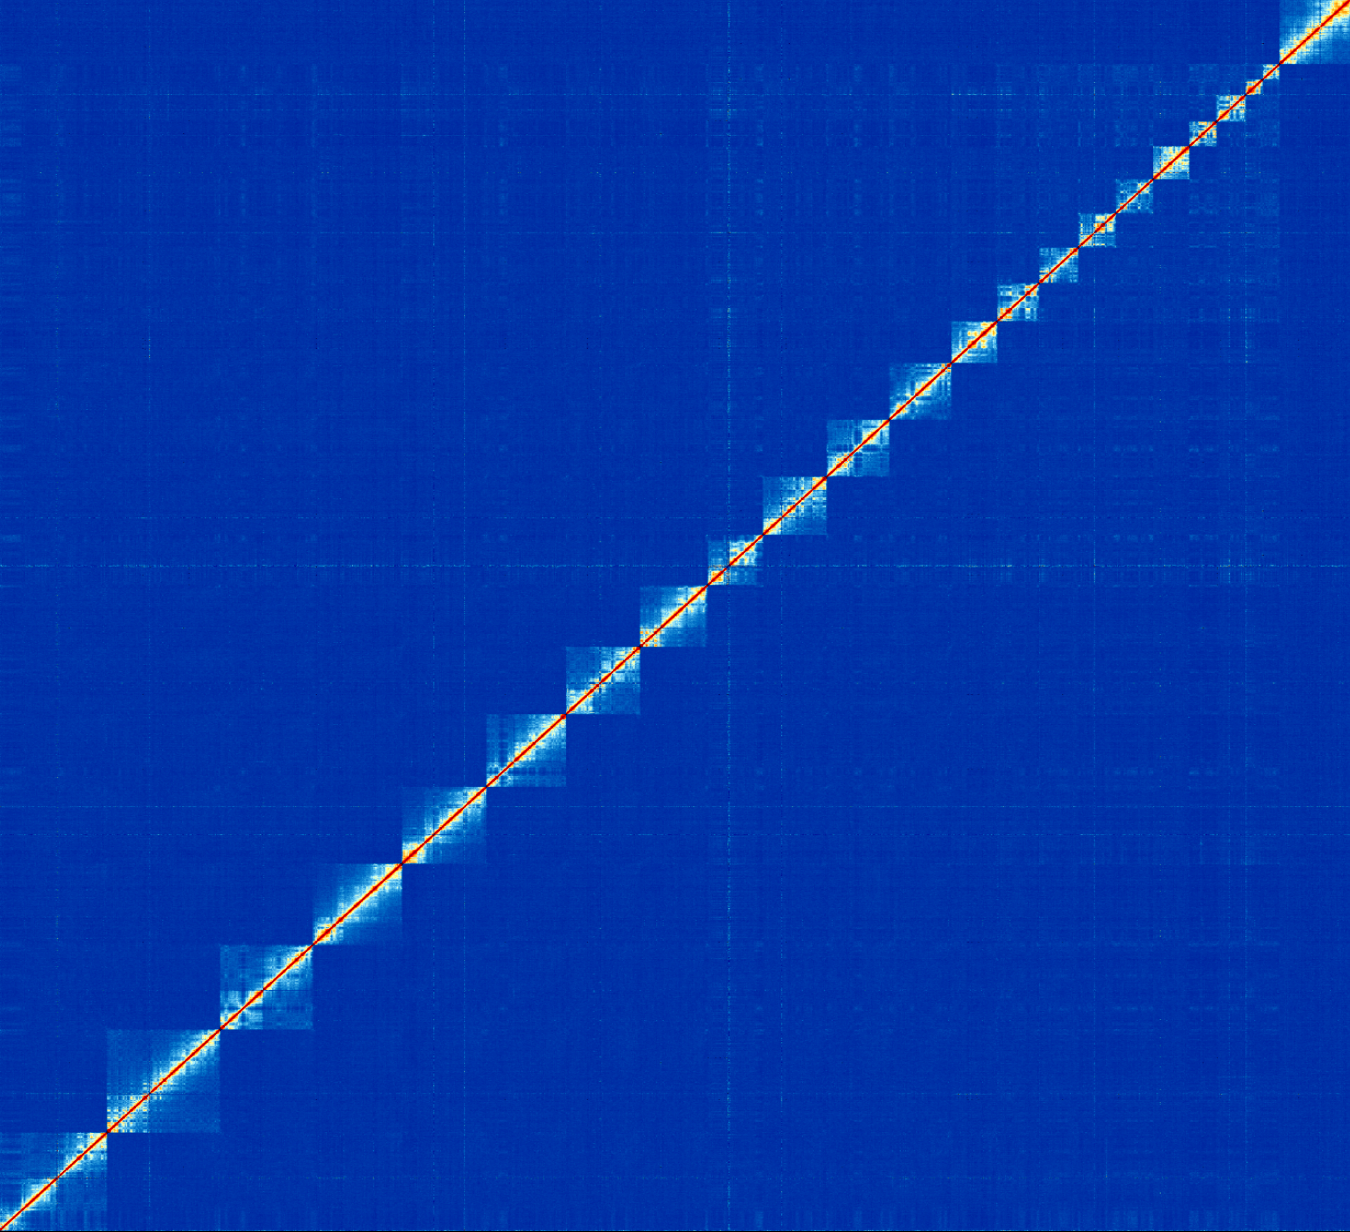
\includegraphics[width=.85\paperwidth]{figs/hicbg_3.png}}
%\setbeamertemplate{sidebar left}{\logo{}}
\begin{frame}
%\hspace{-20em}
\titlepage
\end{frame}
}

% ----- Begin introduction

\section{Introduction}

\begin{frame}{Introduction}

Broad aim: investigate the relationship between structure and function of the genome

\vspace{2em}
Some specific questions:

\begin{enumerate}
\item How does higher order chromatin structure compare across human cell types?
\item Can we predict higher order chromatin structure from locus-level features?
\item How do the characteristics of boundaries demarcating higher order domains vary between cell types and domain classes?
\end{enumerate}

\end{frame}

\begin{frame}{What's known about genome structure}
\centering
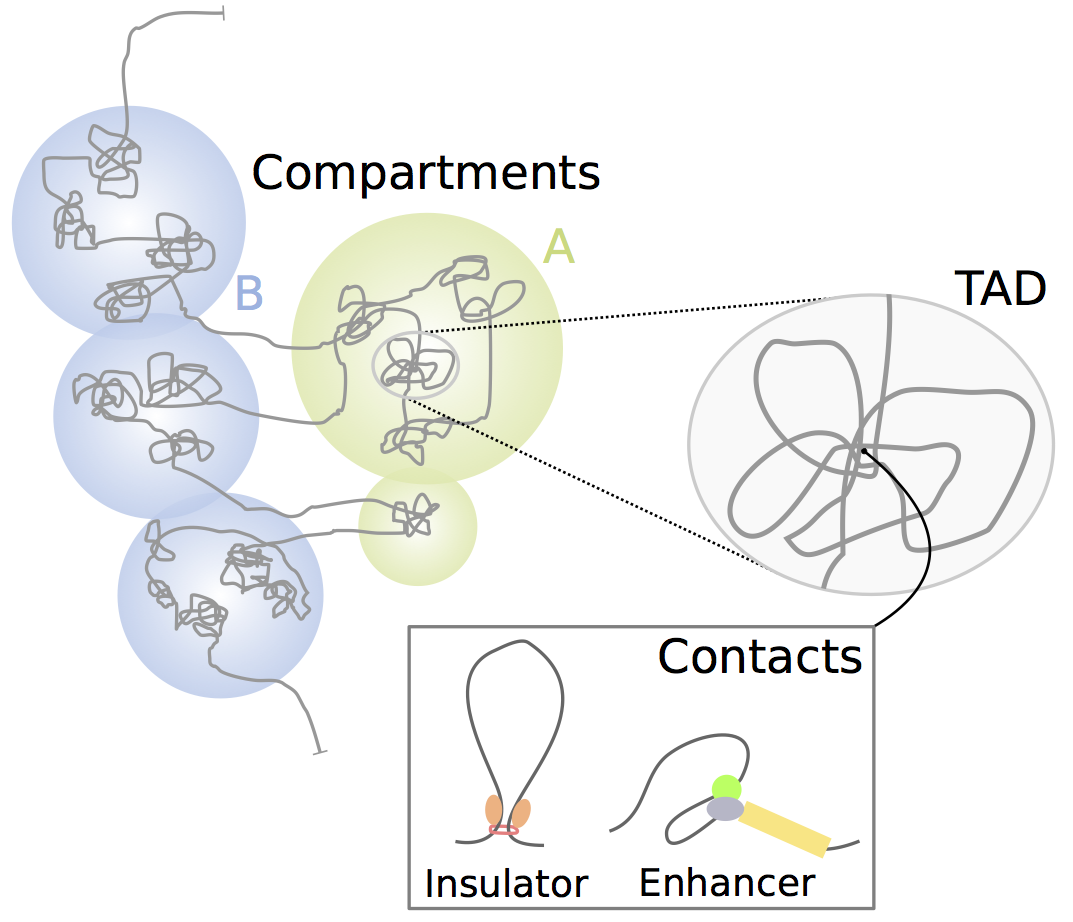
\includegraphics[width=.8\textwidth]{../figs/genome_org.png}

\end{frame}

\begin{frame}{Hi-C: a genome-wide chromosome conformation assay }

\centering
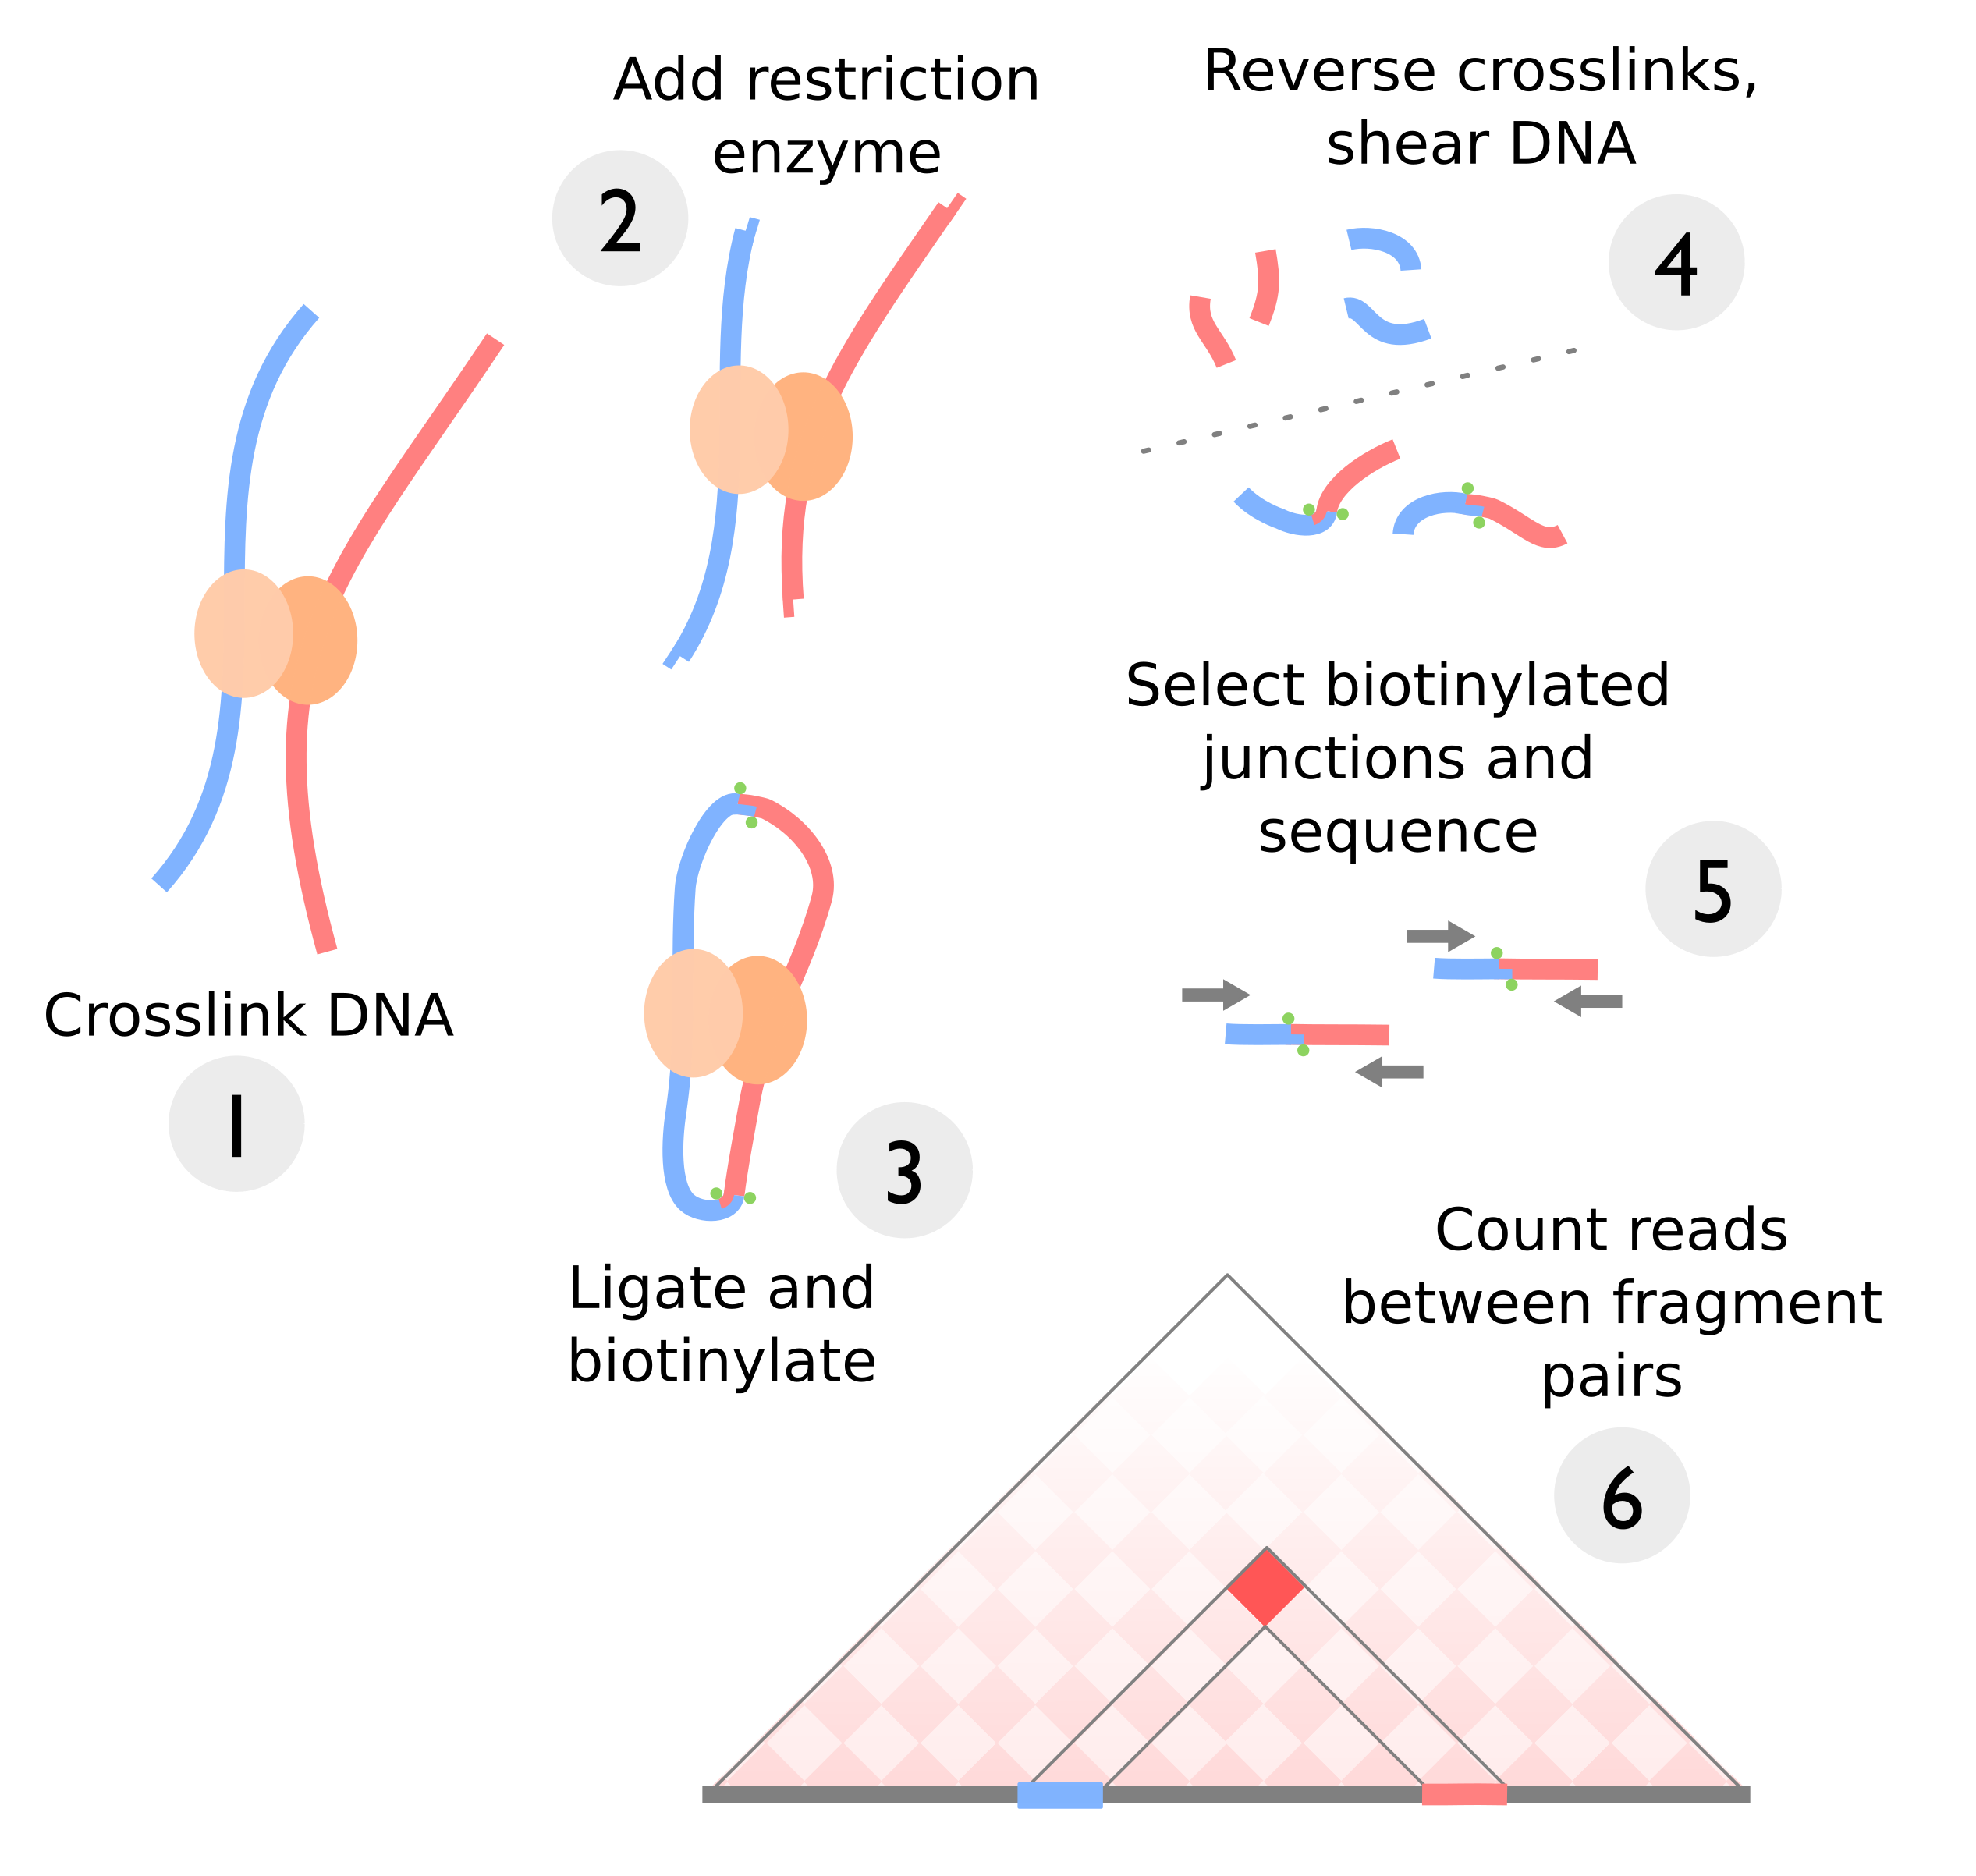
\includegraphics[width=.8\textwidth]{../figs/hic.png}

\end{frame}


\begin{frame}{Chromosome compartments from Hi-C data }

\centering
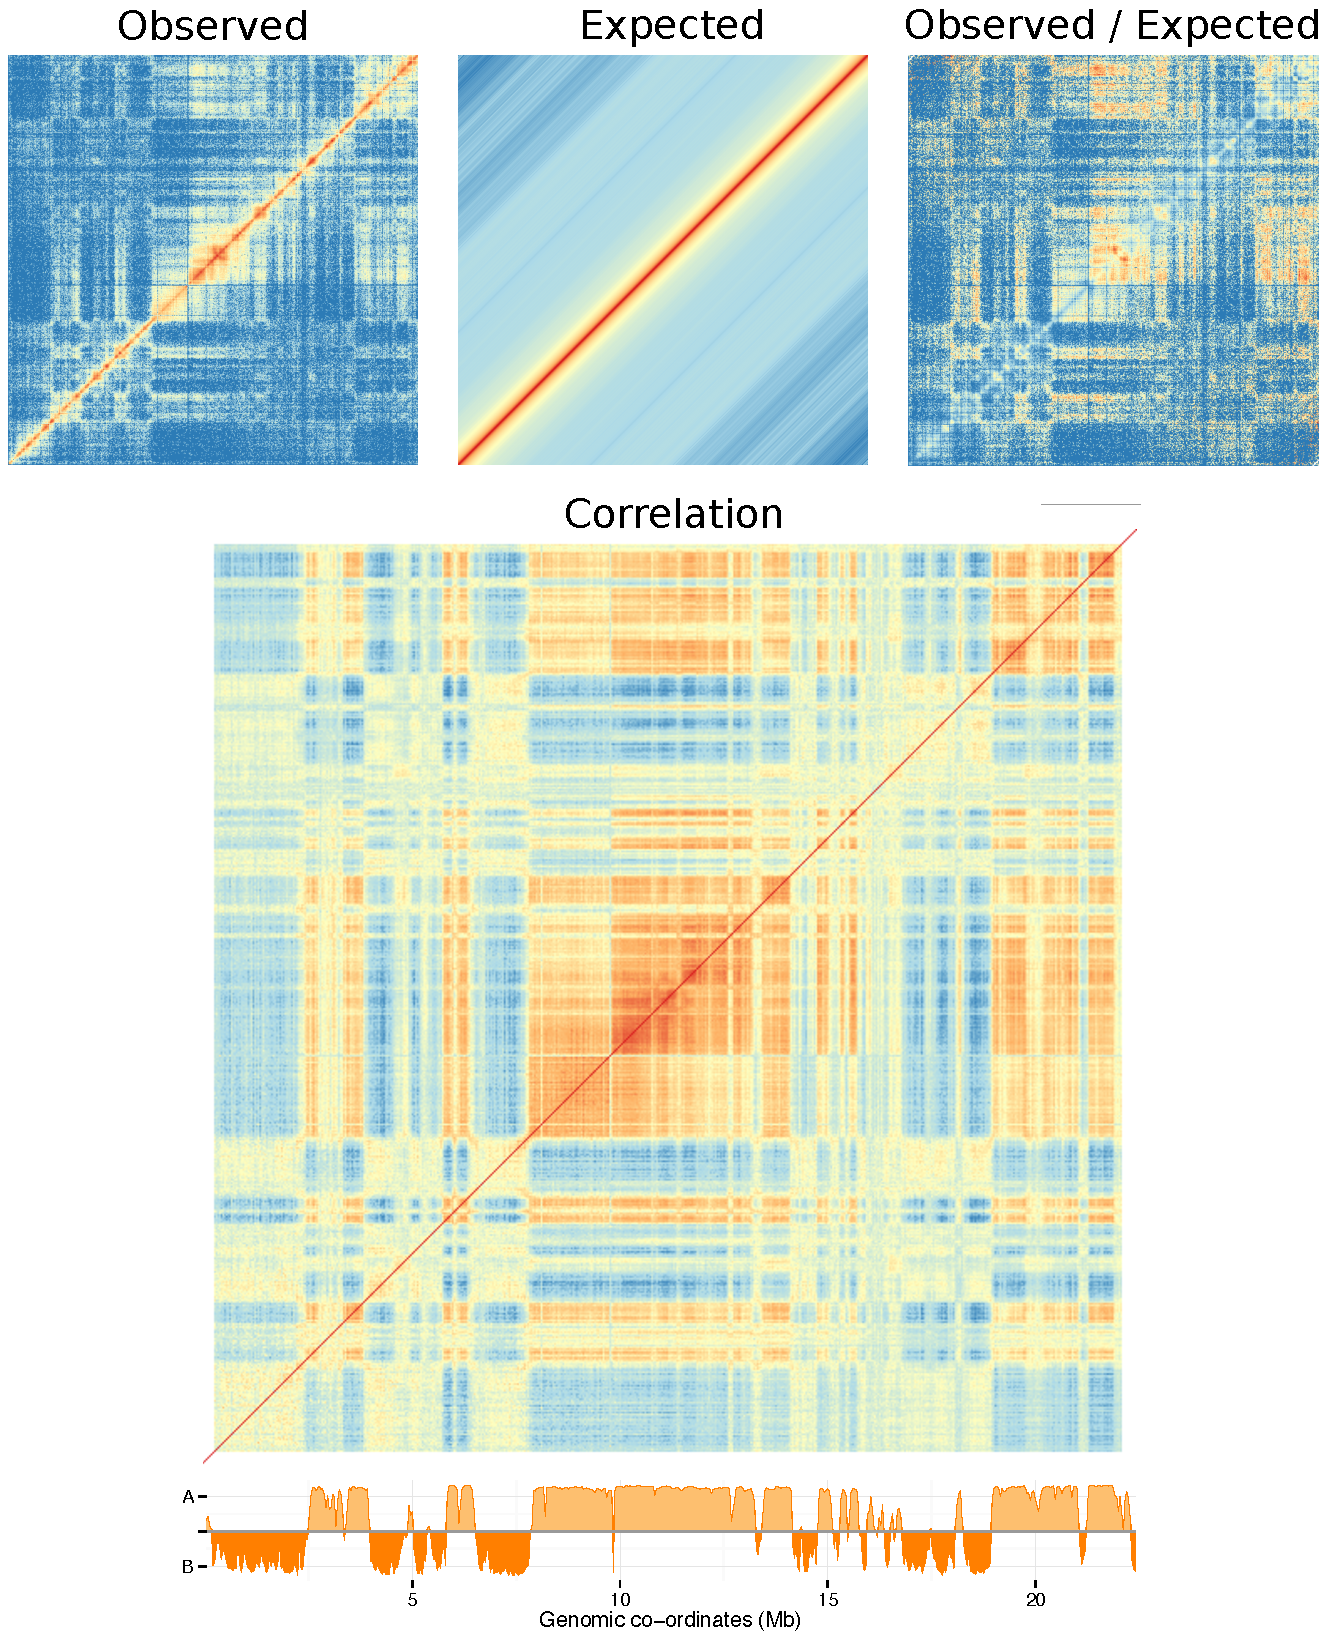
\includegraphics[width=.6\textwidth]{../figs/eigcalc.png}

\end{frame}

\begin{frame}{ Strategy }

{\small

\begin{itemize}
\item Integrate publicly available Hi-C data
\item Uniformly reprocess each dataset 
\item Call compartments, TADs from reprocessed data
\item Integrate cell-matched ENCODE epigenomic data
\end{itemize}

Then:
\begin{enumerate}
\item Compare/contrast cell types after reprocessing
\item Attempt predictive models of compartments and TADs from epigenomic features
\item Analyse boundary composition in terms of epigenomic features
\end{enumerate}

Related collaborative work:
\begin{enumerate}
\setcounter{enumi}{3}
\item Investigate concept of "metaTADs"
\item Analyse conformation changes at specific locus of interest 
\end{enumerate}
}

\end{frame}

% ----- End of introduction

% ----- Begin Reanalysis of Hi-C

\section{Reanalysis of Hi-C datasets}

{
\usebackgroundtemplate{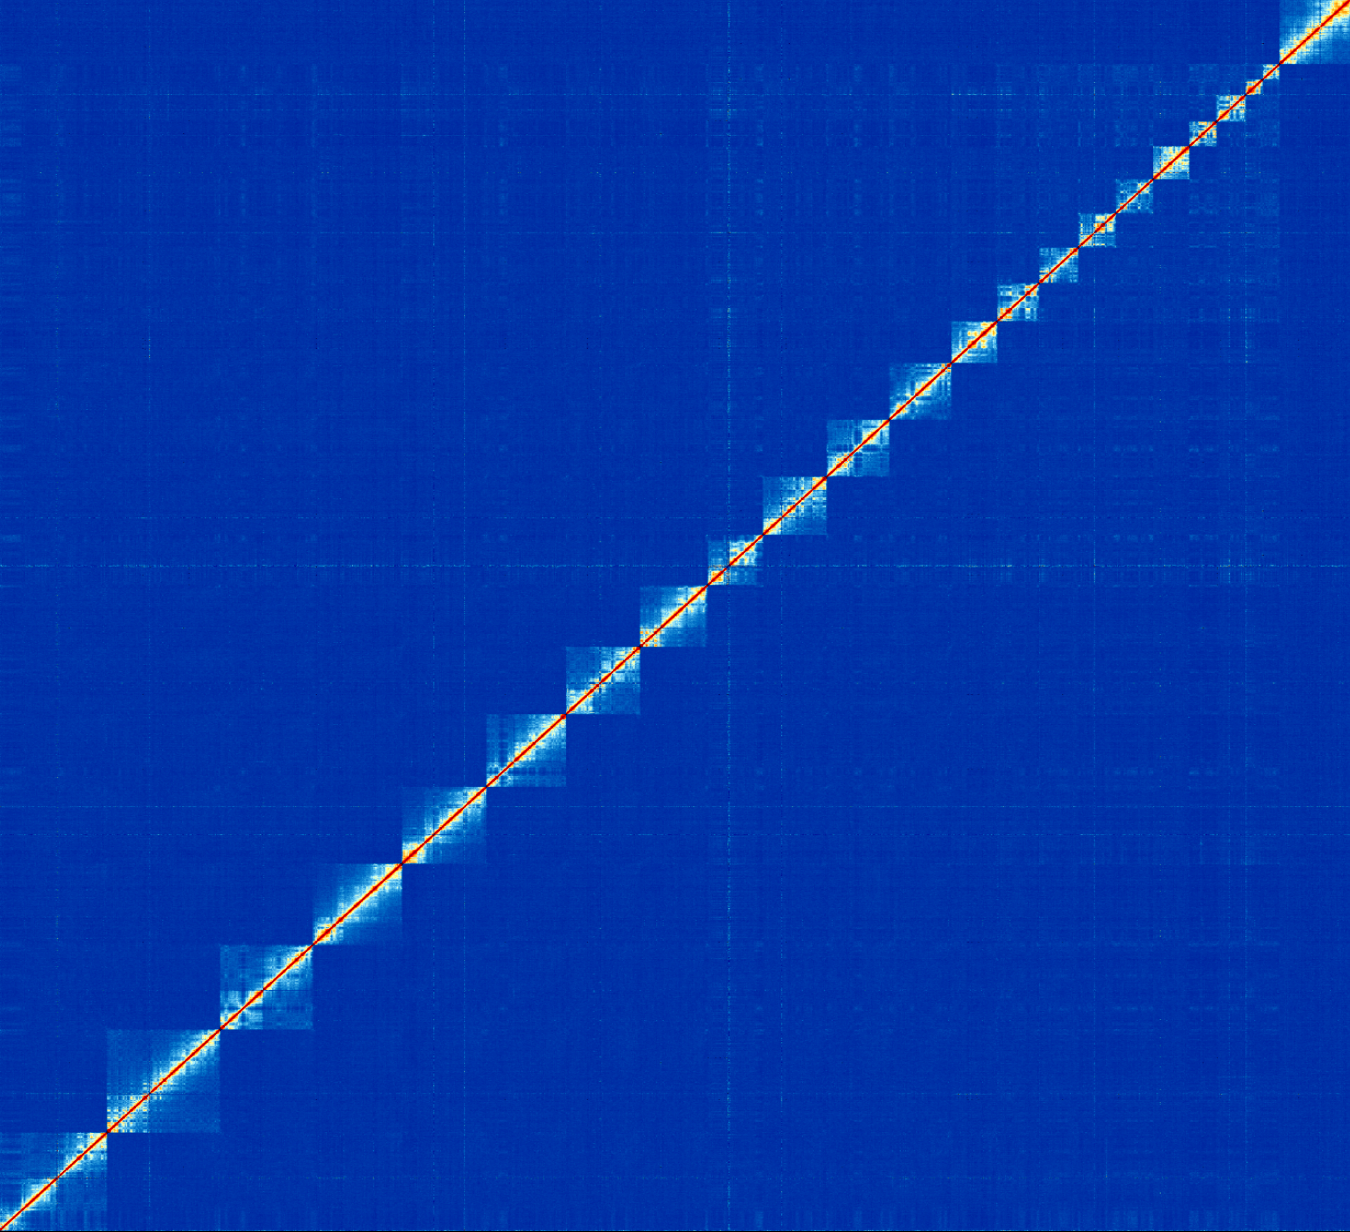
\includegraphics[width=.85\paperwidth]{figs/hicbg_3.png}}
\begin{frame}{}
\begin{tcolorbox}[colback=blue!40!black,colframe=blue!40!black]
\begin{center}
{\usebeamercolor[fg]{whitetext}
{\small Results 1: } \\
 Reanalysis of Hi-C data }
\end{center}
\end{tcolorbox}
\end{frame}
}

\begin{frame}{Reanalysis of Hi-C datasets}
Very different sequencing depths between the input datasets: \\

\vspace{2em}

\centering
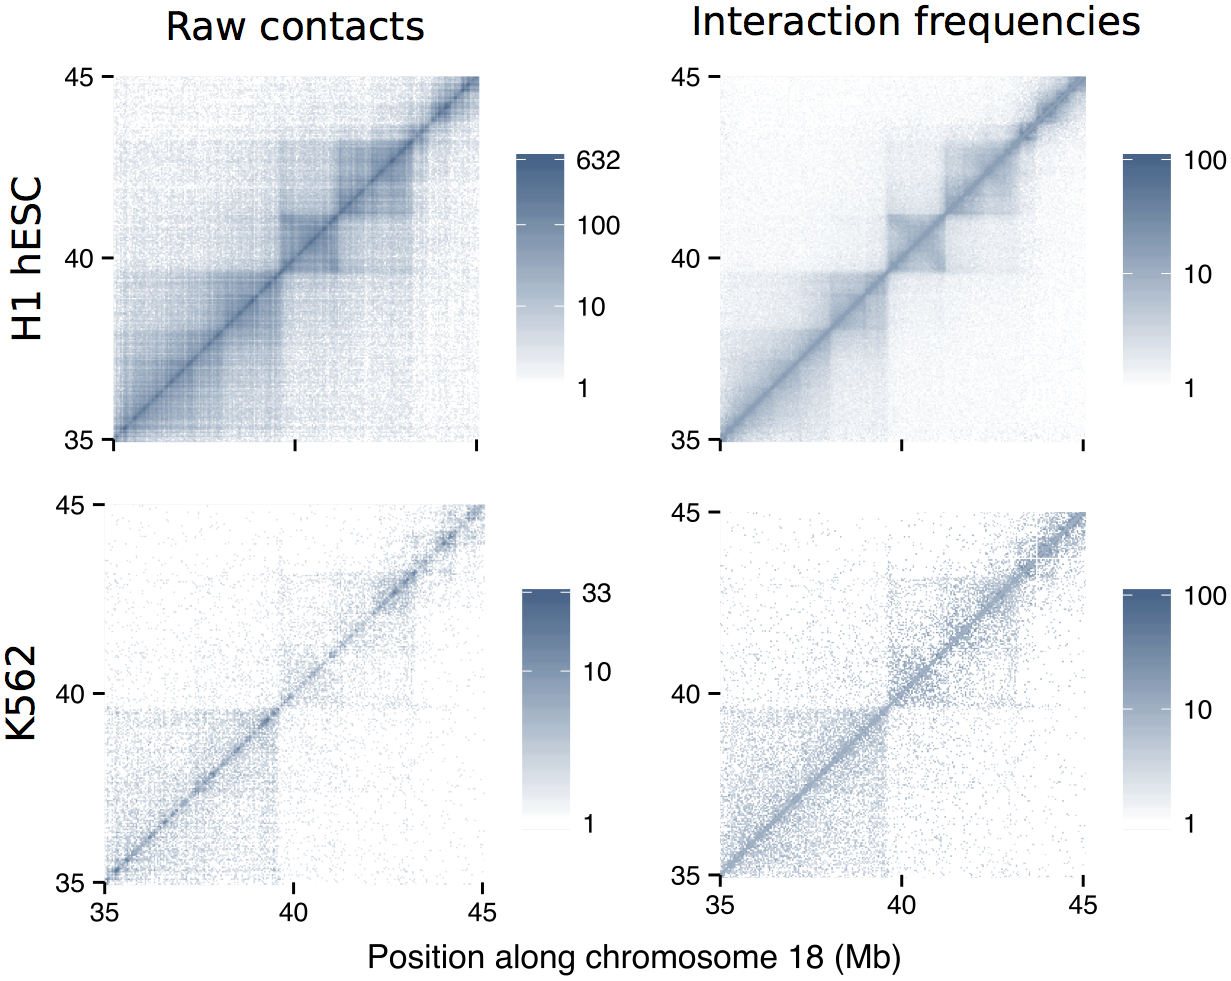
\includegraphics[width=.9\textwidth]{../figs/hicnorm.png}

\end{frame}

\begin{frame}{Reanalysis of Hi-C datasets}
Despite this, reprocessed Hi-C data is well-correlated: \\

\vspace{2em}

{\centering
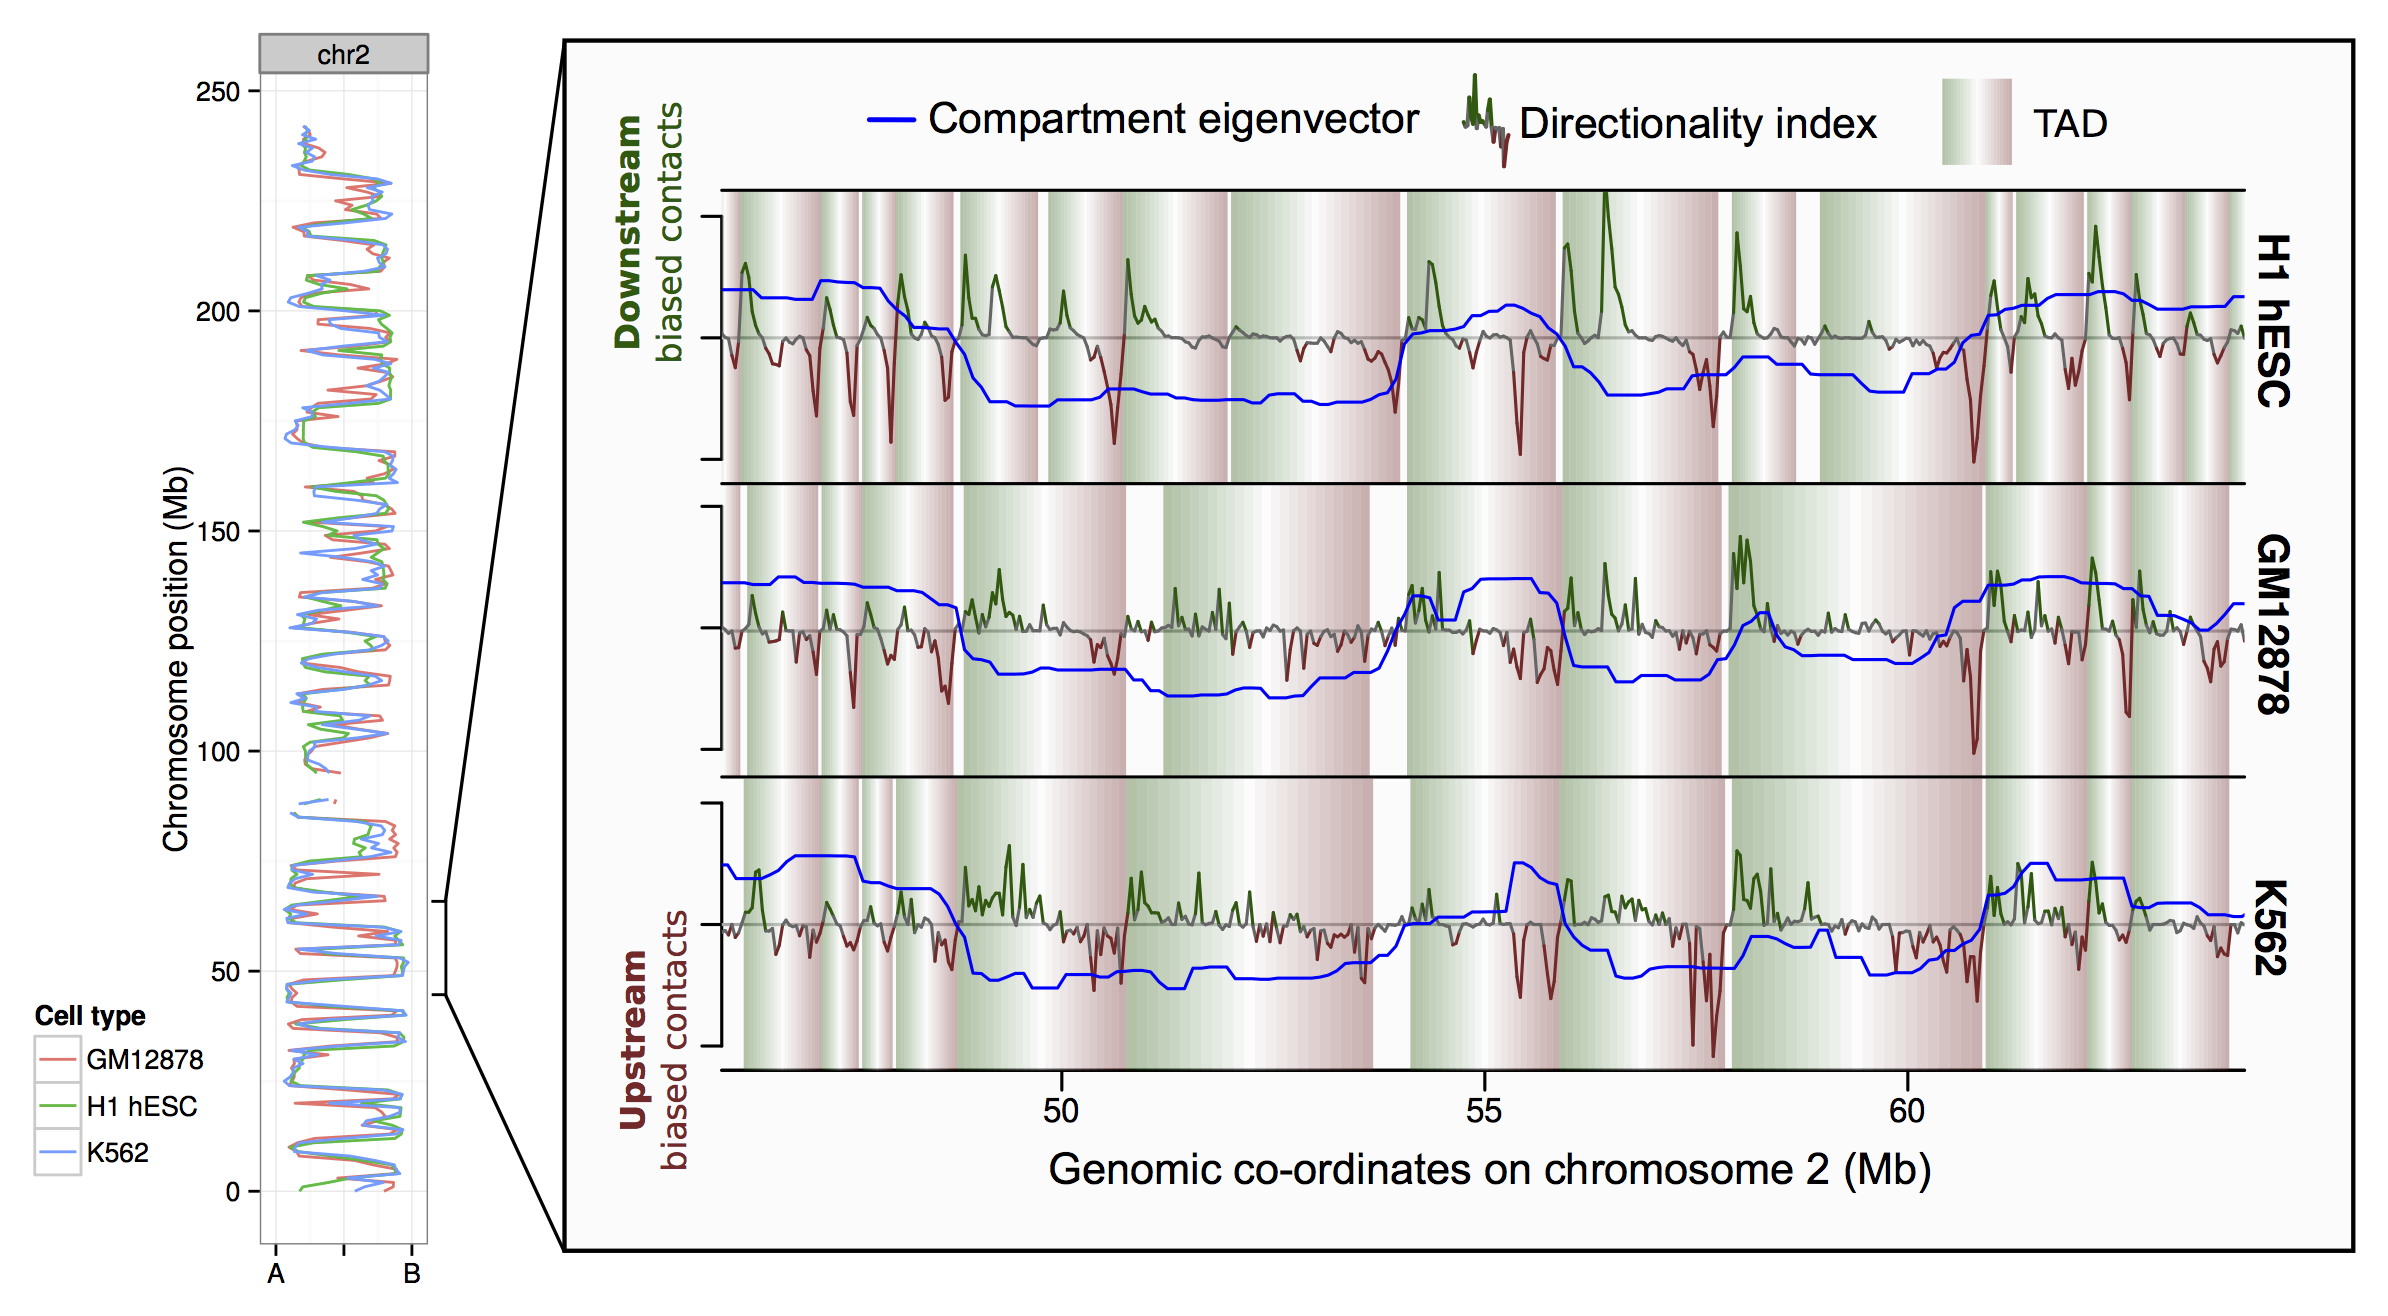
\includegraphics[width=.9\textwidth]{../figs/blowout.png}
}
\vspace{2em}

Justifies going forward with between cell-line analysis

\end{frame}

\begin{frame}{Improved compartment calling algorithm}

\begin{columns}

\column{.4\textwidth}
\centering
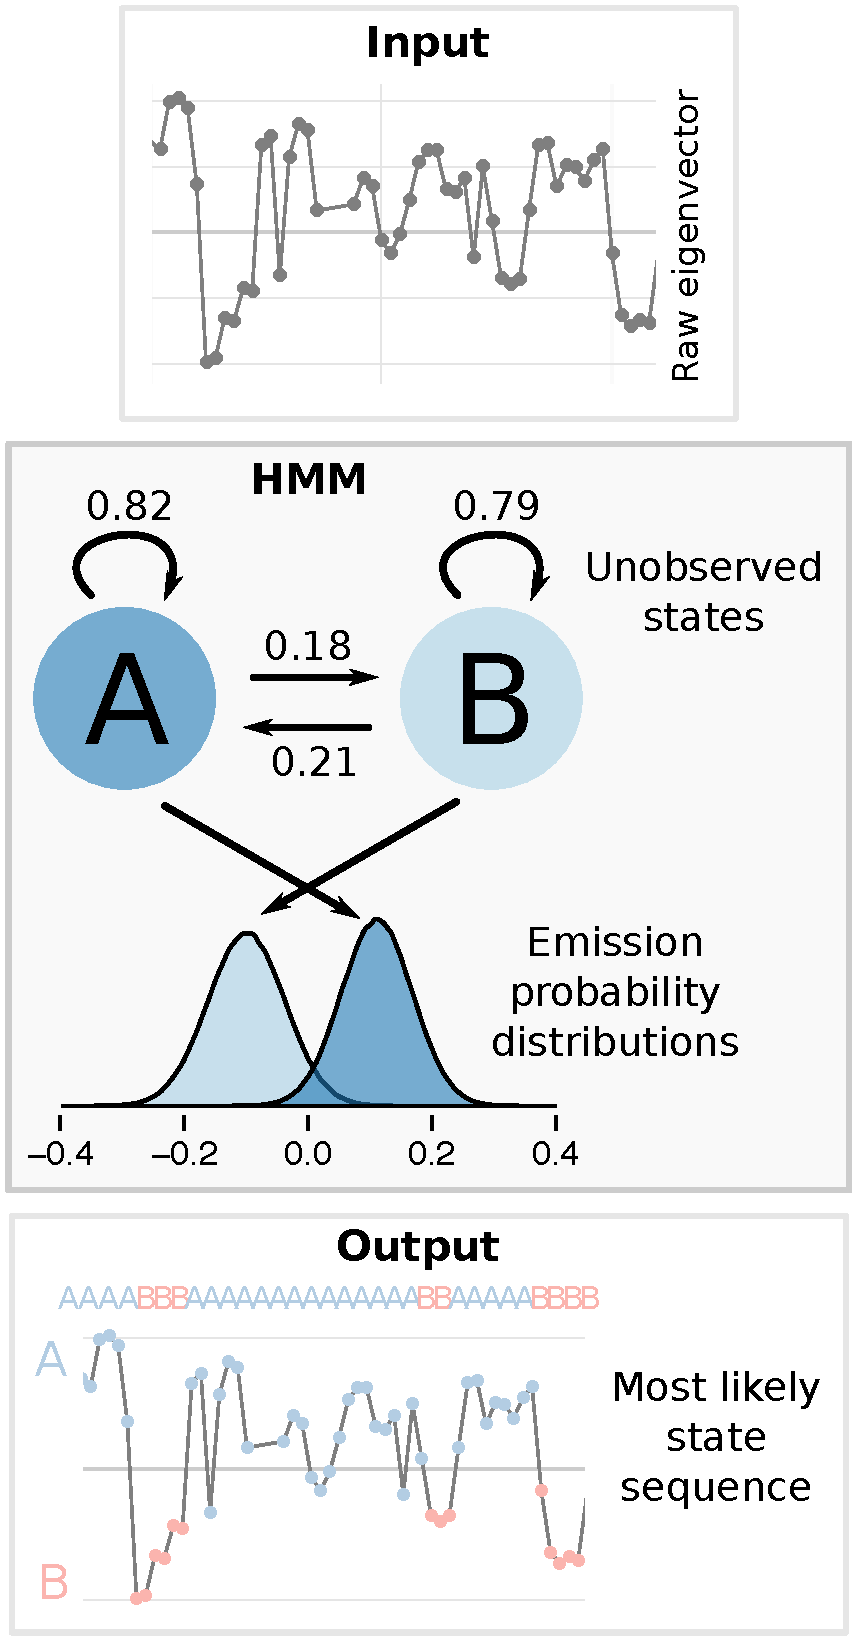
\includegraphics[width=.85\textwidth]{../figs/hmm_flow.pdf}

\column{.6\textwidth}
\centering
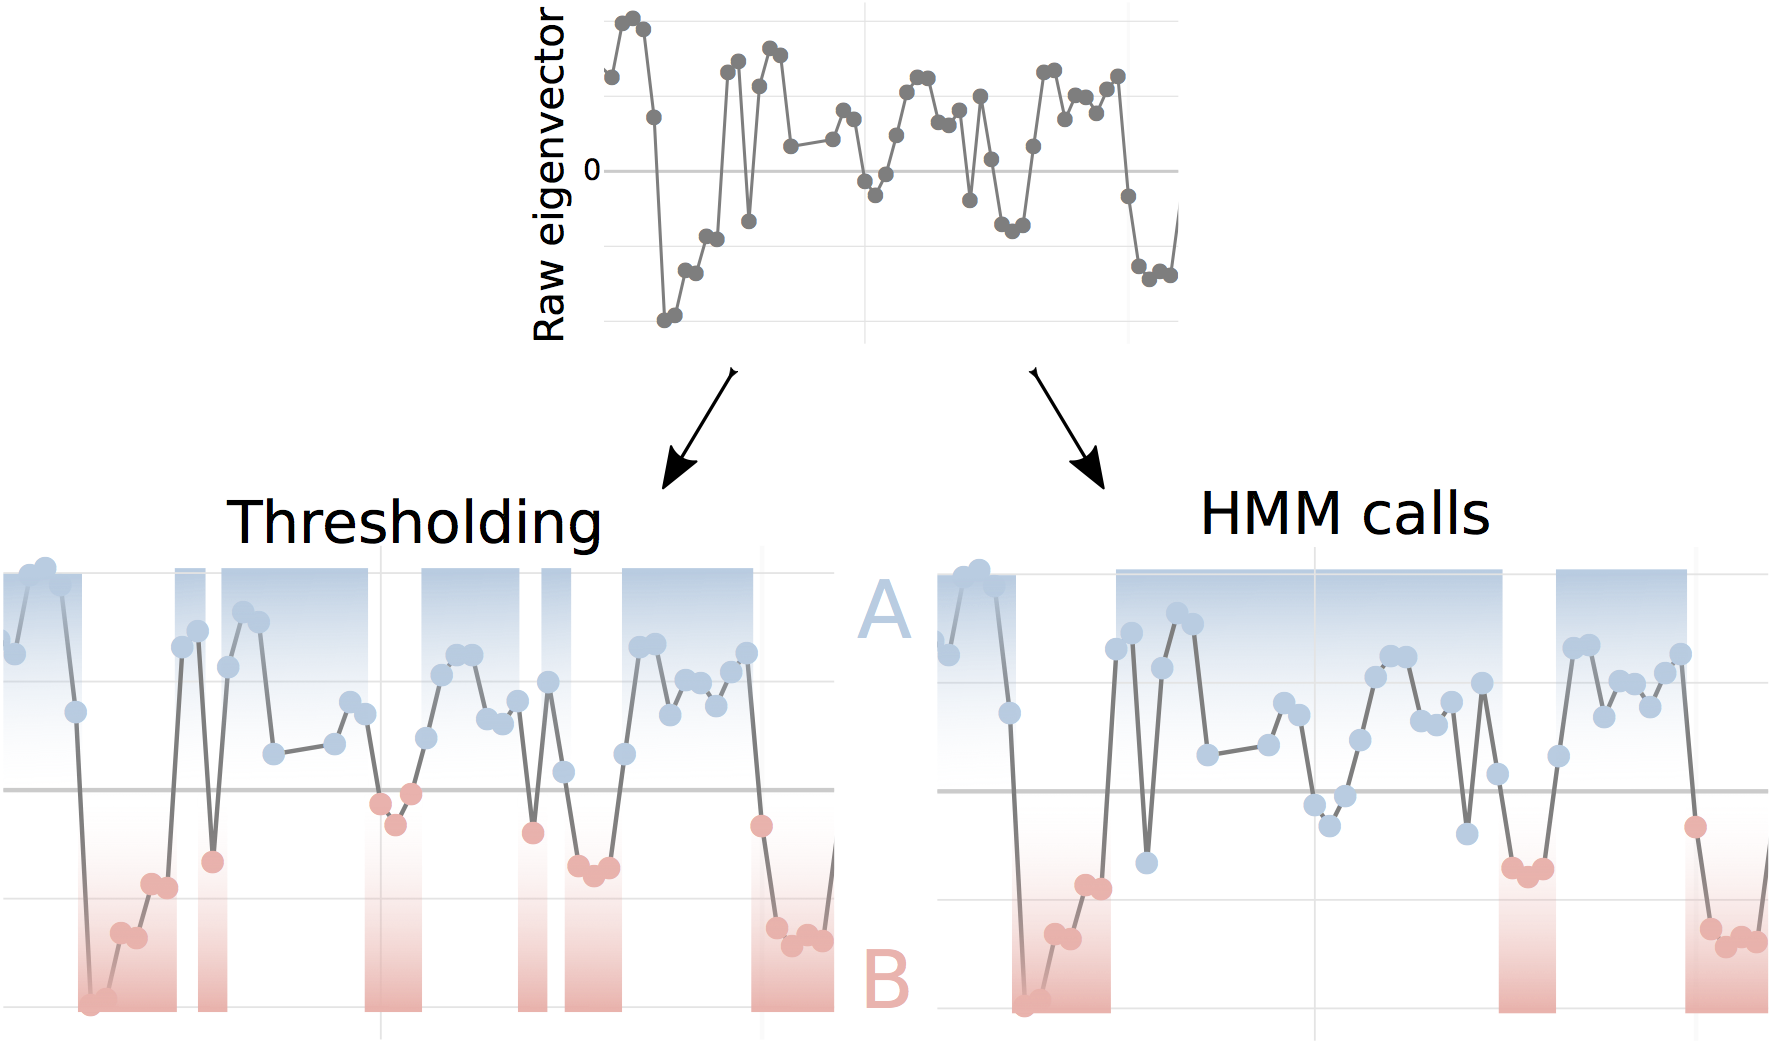
\includegraphics[width=\textwidth]{../figs/hmm_calls.png}

\end{columns}

\end{frame}

\begin{frame}{Regions of variable compartment structure}

Regions of open, active compartment in one cell type but closed, repressive in the other two are enriched for cell type specific enhancer chromatin states: \\

\vspace{2em}

\centering
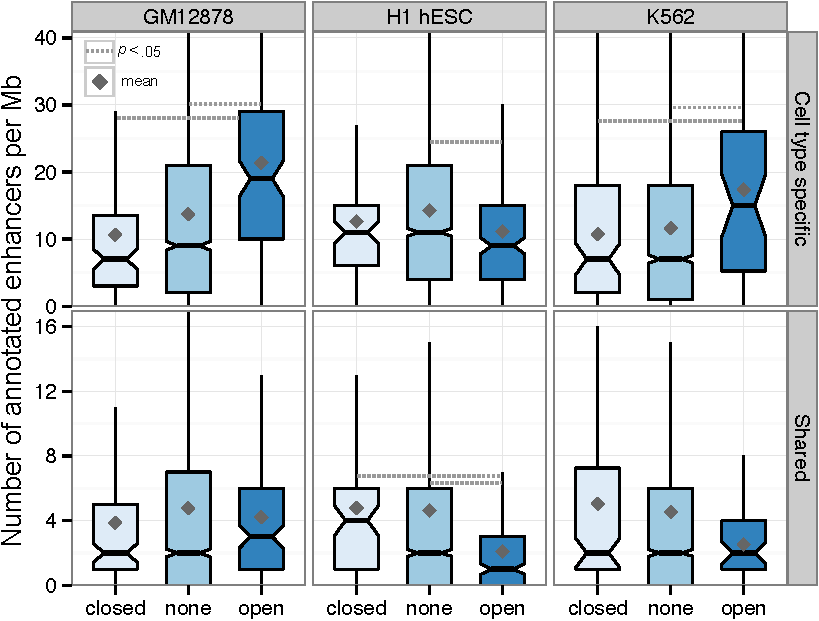
\includegraphics[width=.55\textwidth]{../figs/enhancerstates.pdf}

\end{frame}

\begin{frame}{Regions of variable compartment structure}

Some harbour genes with known cell type specific function

\vspace{1em}

\centering
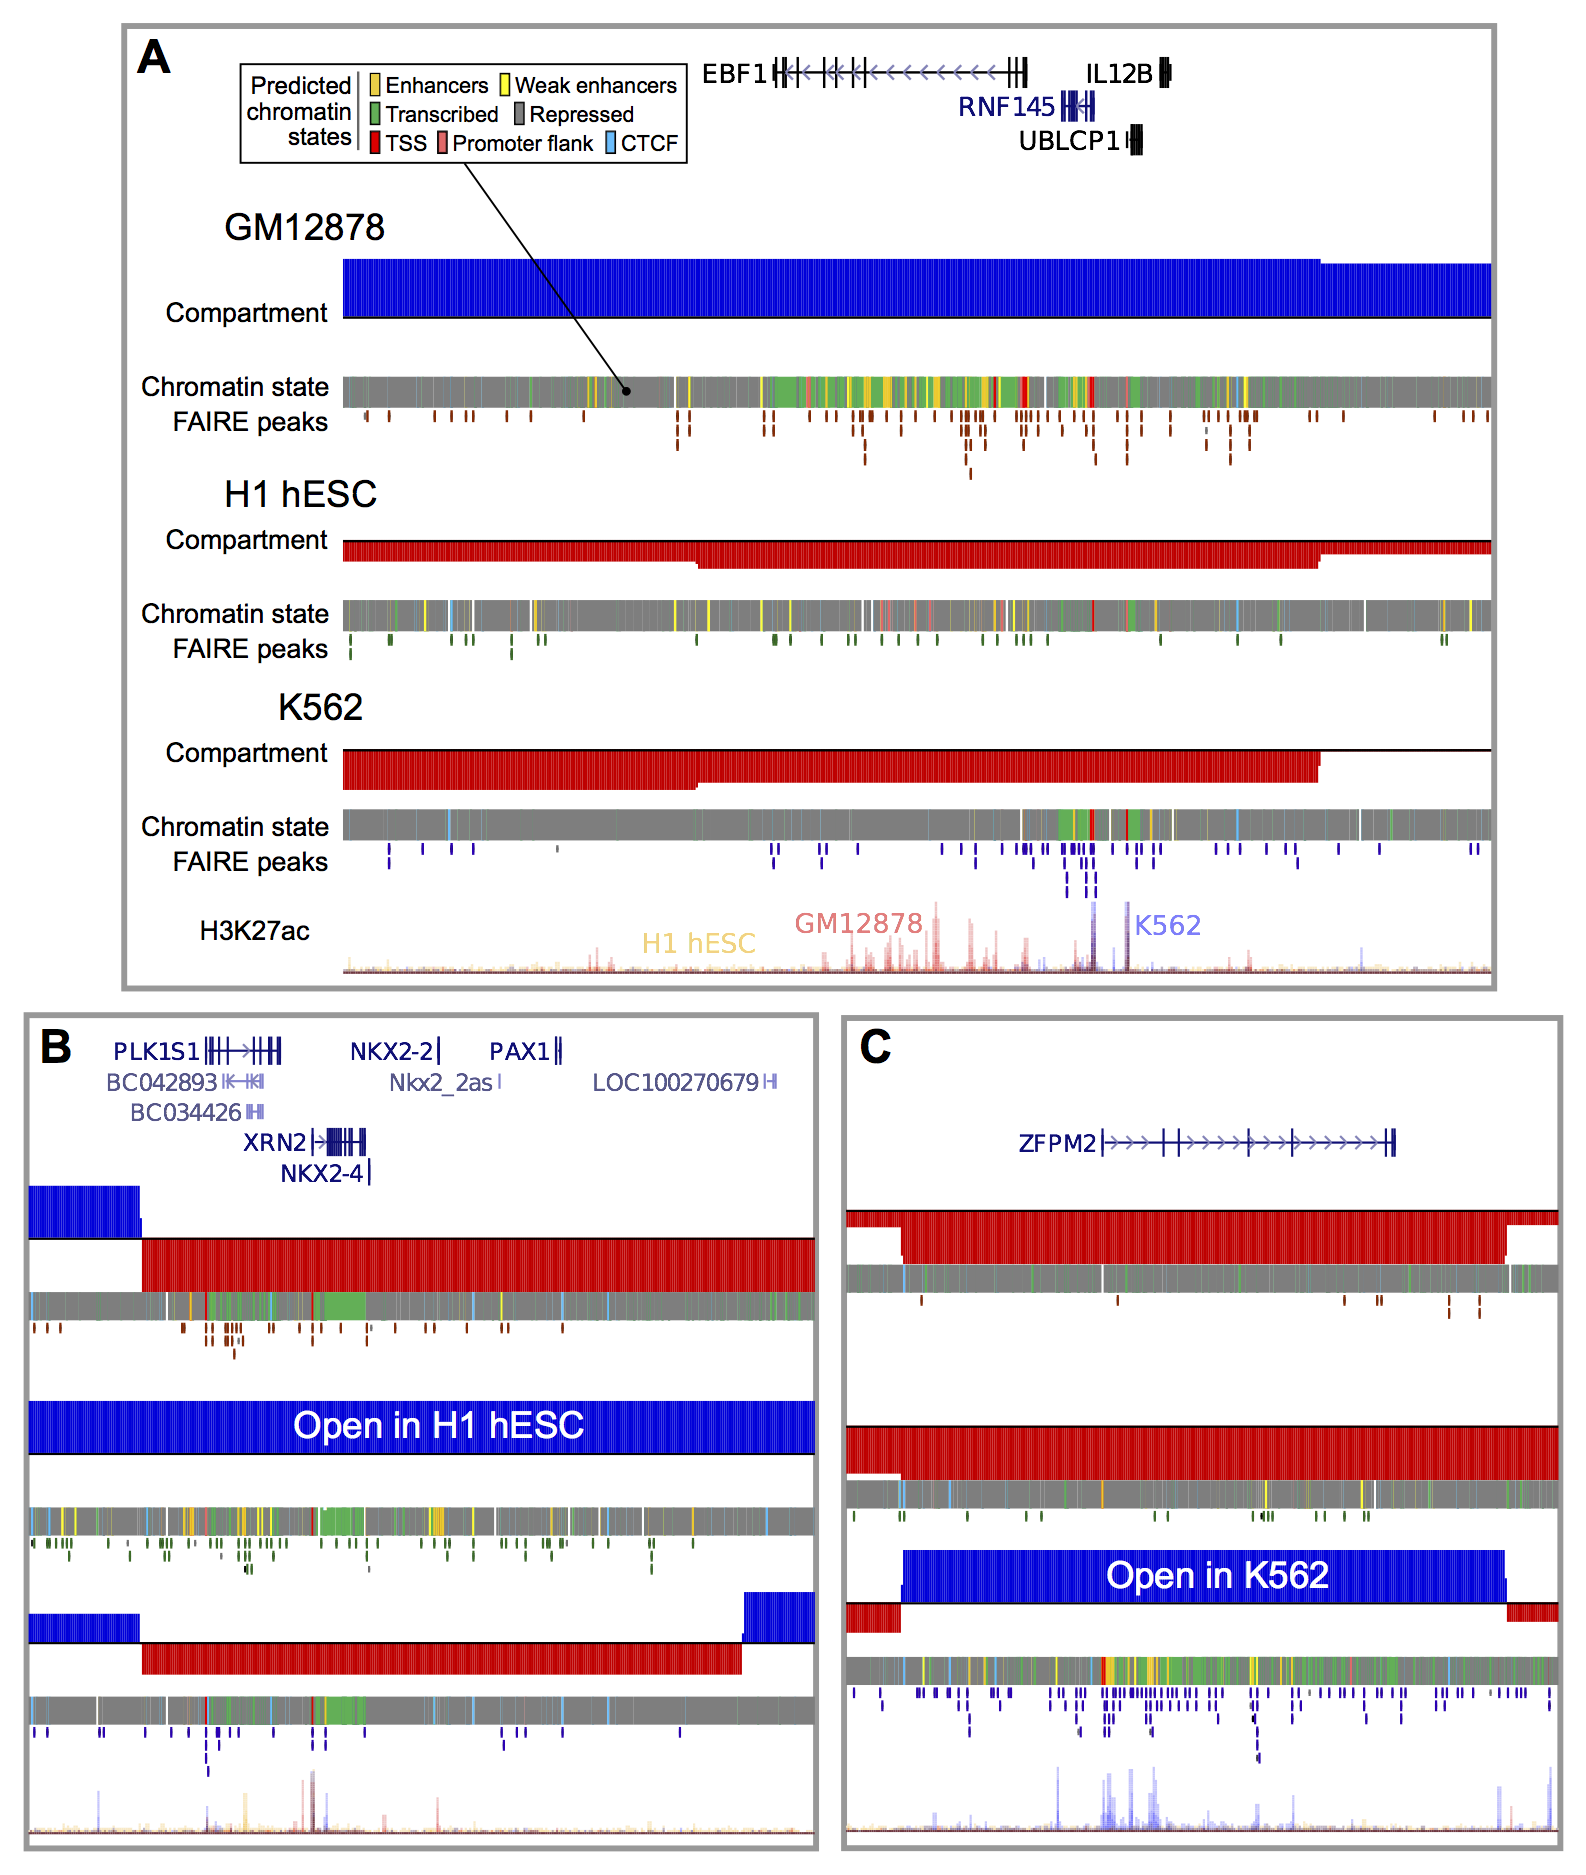
\includegraphics[width=.55\textwidth]{../figs/examplervs.png}

\end{frame}



% ----- End Reanalysis of Hi-C

\section{Integrative modelling}

{
\usebackgroundtemplate{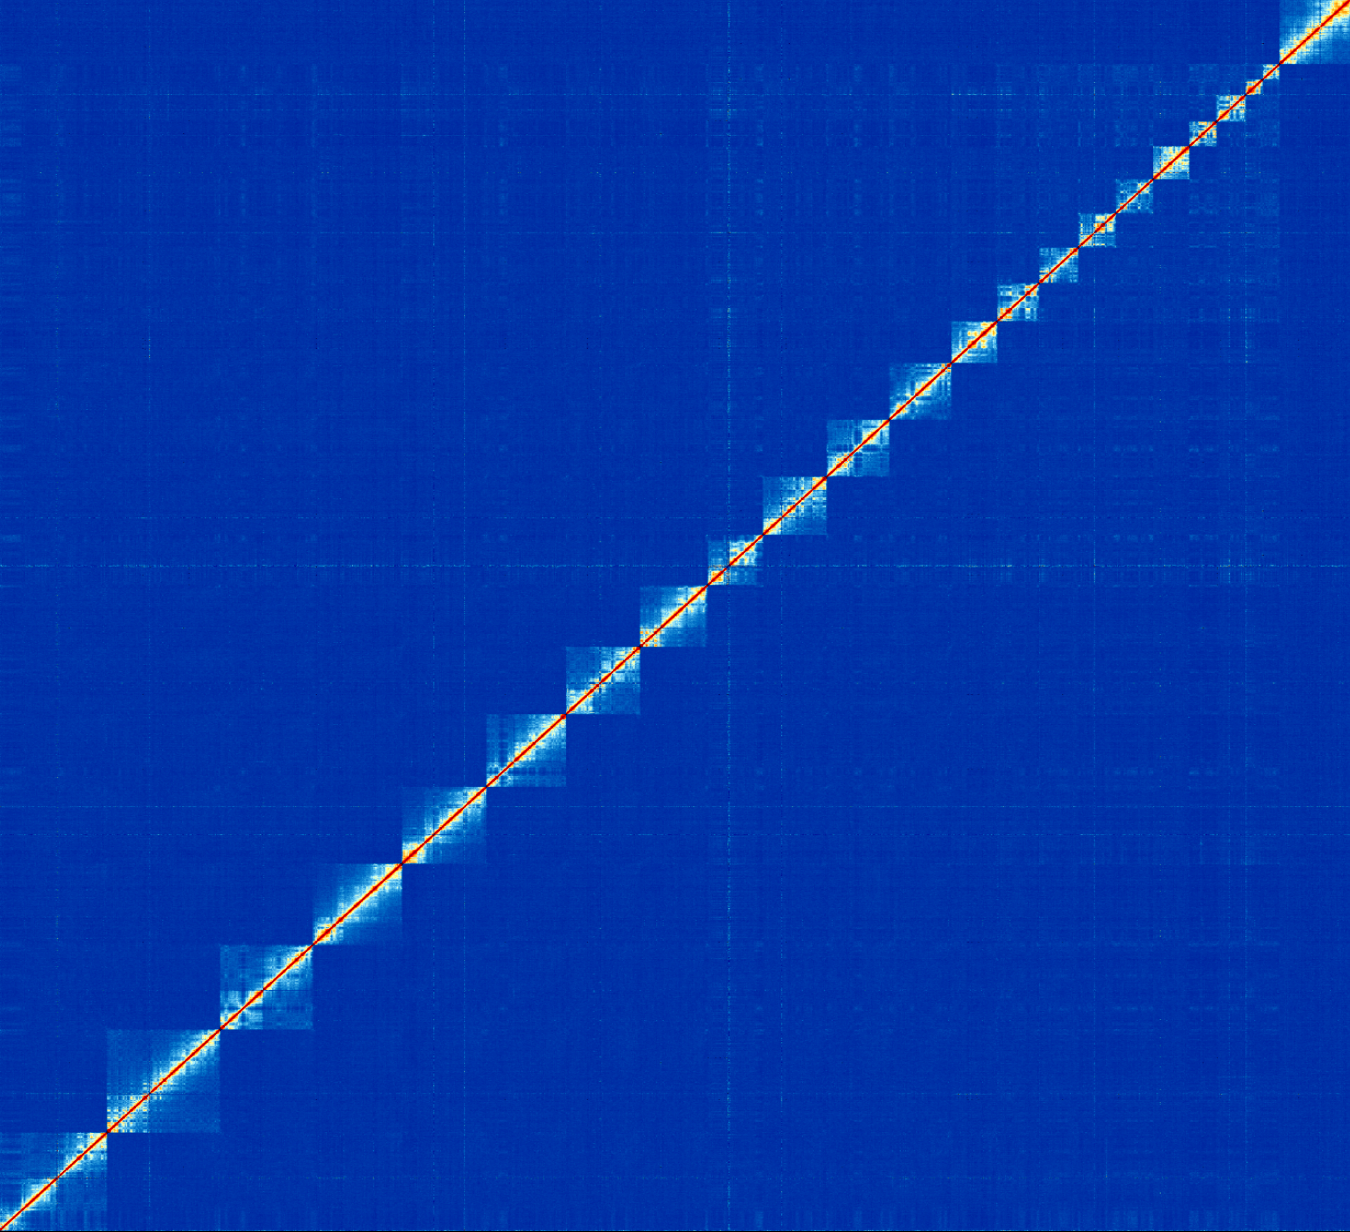
\includegraphics[width=.85\paperwidth]{figs/hicbg_3.png}}
\begin{frame}{}
\begin{tcolorbox}[colback=blue!40!black,colframe=blue!40!black]
\begin{center}
{\usebeamercolor[fg]{whitetext}
{\small Results 2: } \\
 Integrative modelling as a tool \\ to explore biological systems}
\end{center}
\end{tcolorbox}
\end{frame}
}

% ----- Begin Integrative modelling

\begin{frame}{Integrative modelling}{p67}

Chromosome compartment profiles can be accurately predicted and models generalise across cell types: \\

\vspace{2em}

\centering
\includegraphics[width=.65\textwidth]{figs/f2.png}
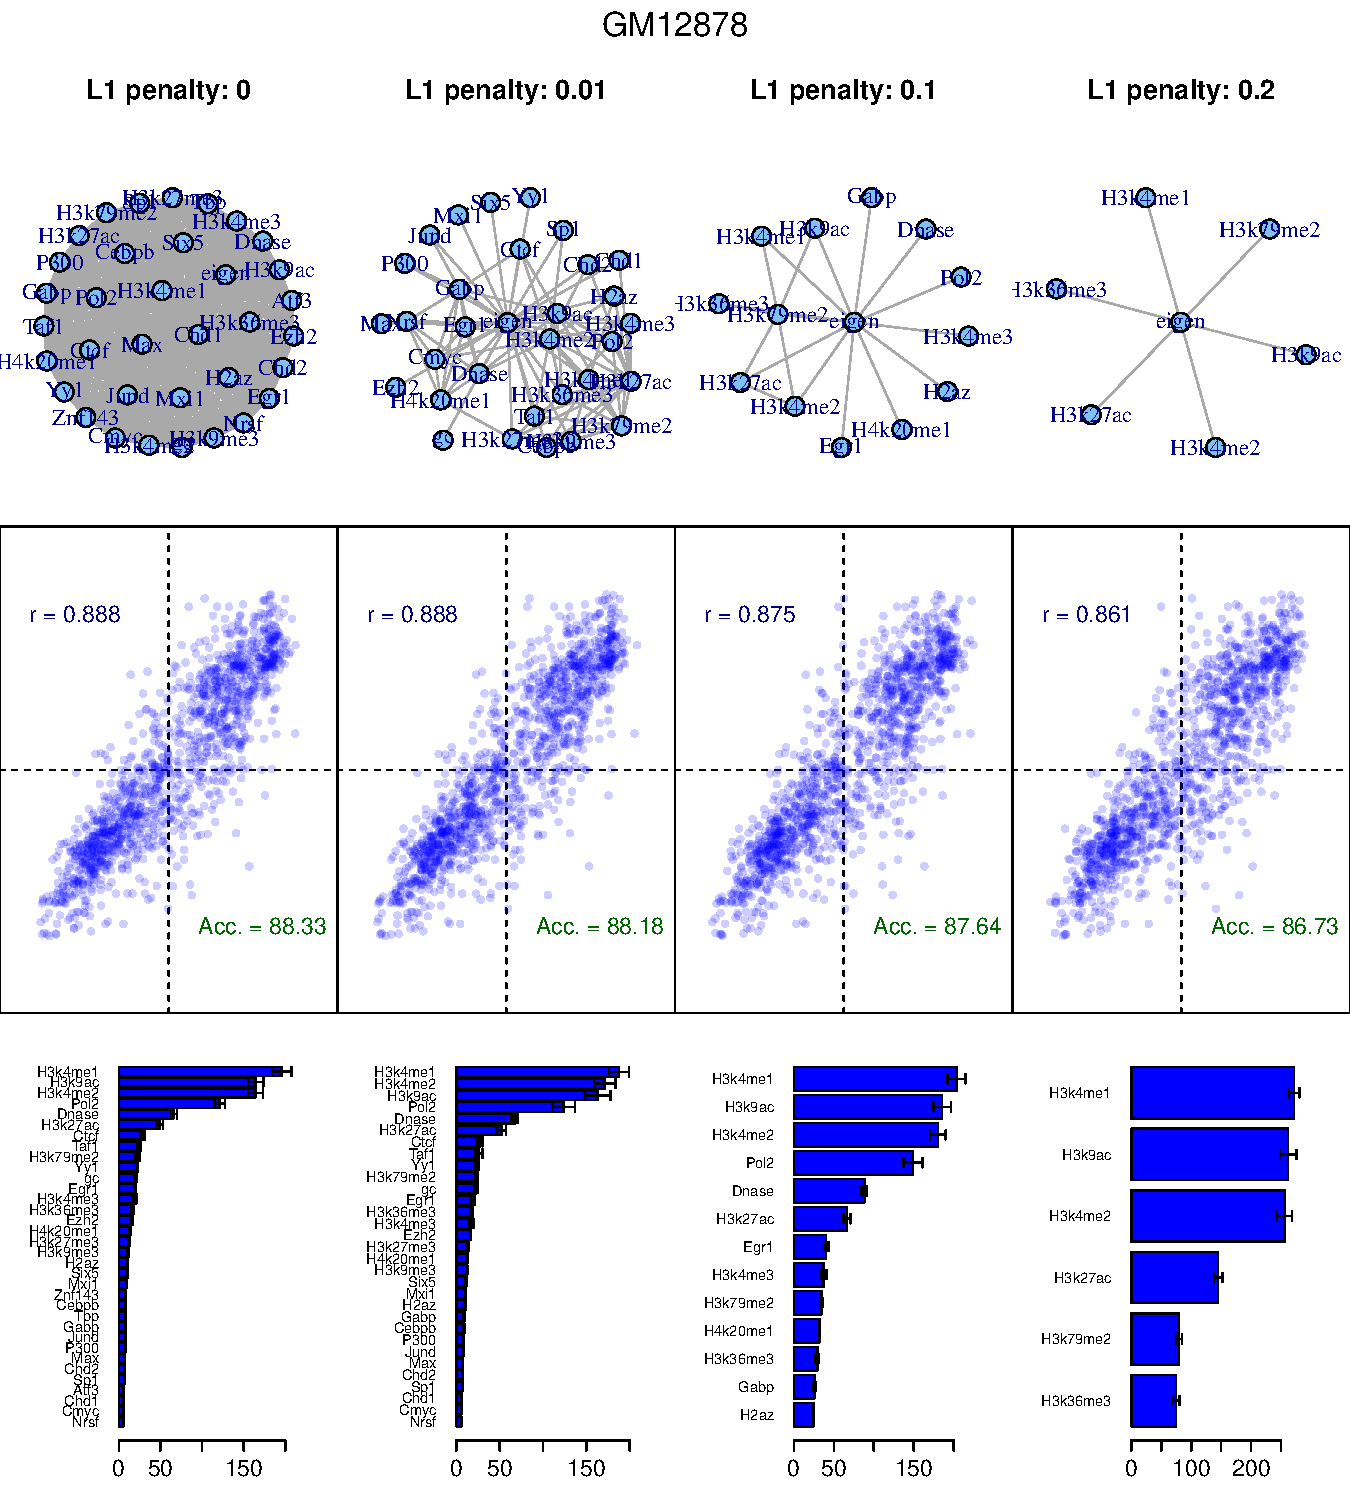
\includegraphics[width=.35\textwidth]{figs/f3.png}

\end{frame}

\begin{frame}{Integrative modelling}

Model dissection a focus of much of this chapter: \\

\vspace{2em}

\begin{itemize}
\item Variable importance
\begin{itemize}
\item Varies between cell type models but multicollinearity in feature set
\item In some cases interpretable (p70), many of the usual suspects of chromatin conformation
\end{itemize}
\item Comparing machine learning methods
\item Regularised models
\end{itemize}

\vspace{1em}

\end{frame}

\begin{frame}{Integrative modelling}

Most results in these two chapters were published:

\vspace{2em}
\centering
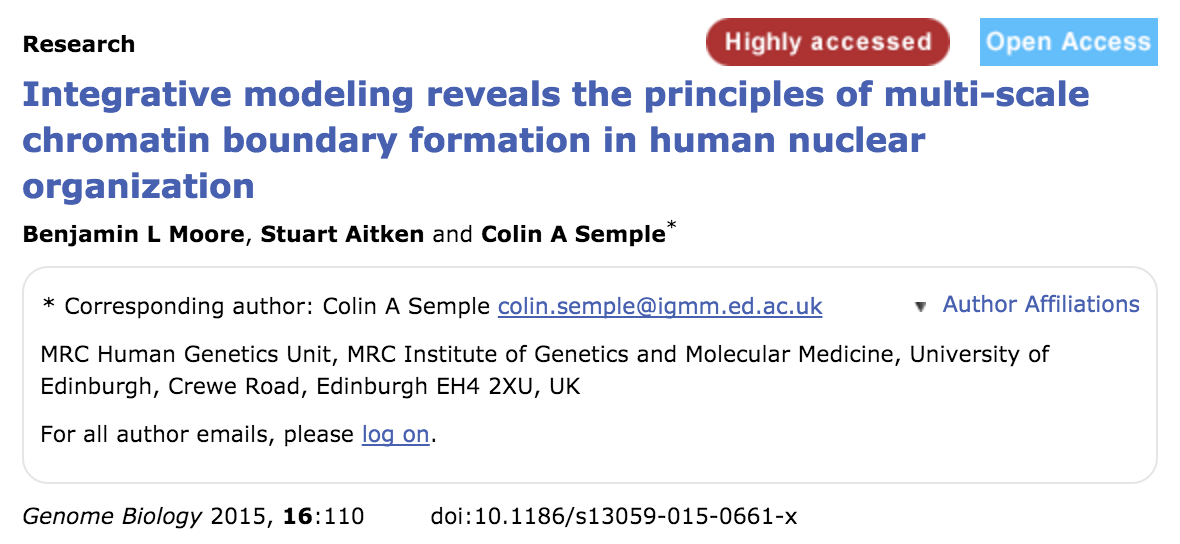
\includegraphics[width=.9\textwidth]{../figs/paper_screenshot.png}
\vspace{2em}

\end{frame}

\section{Boundaries}

{
\usebackgroundtemplate{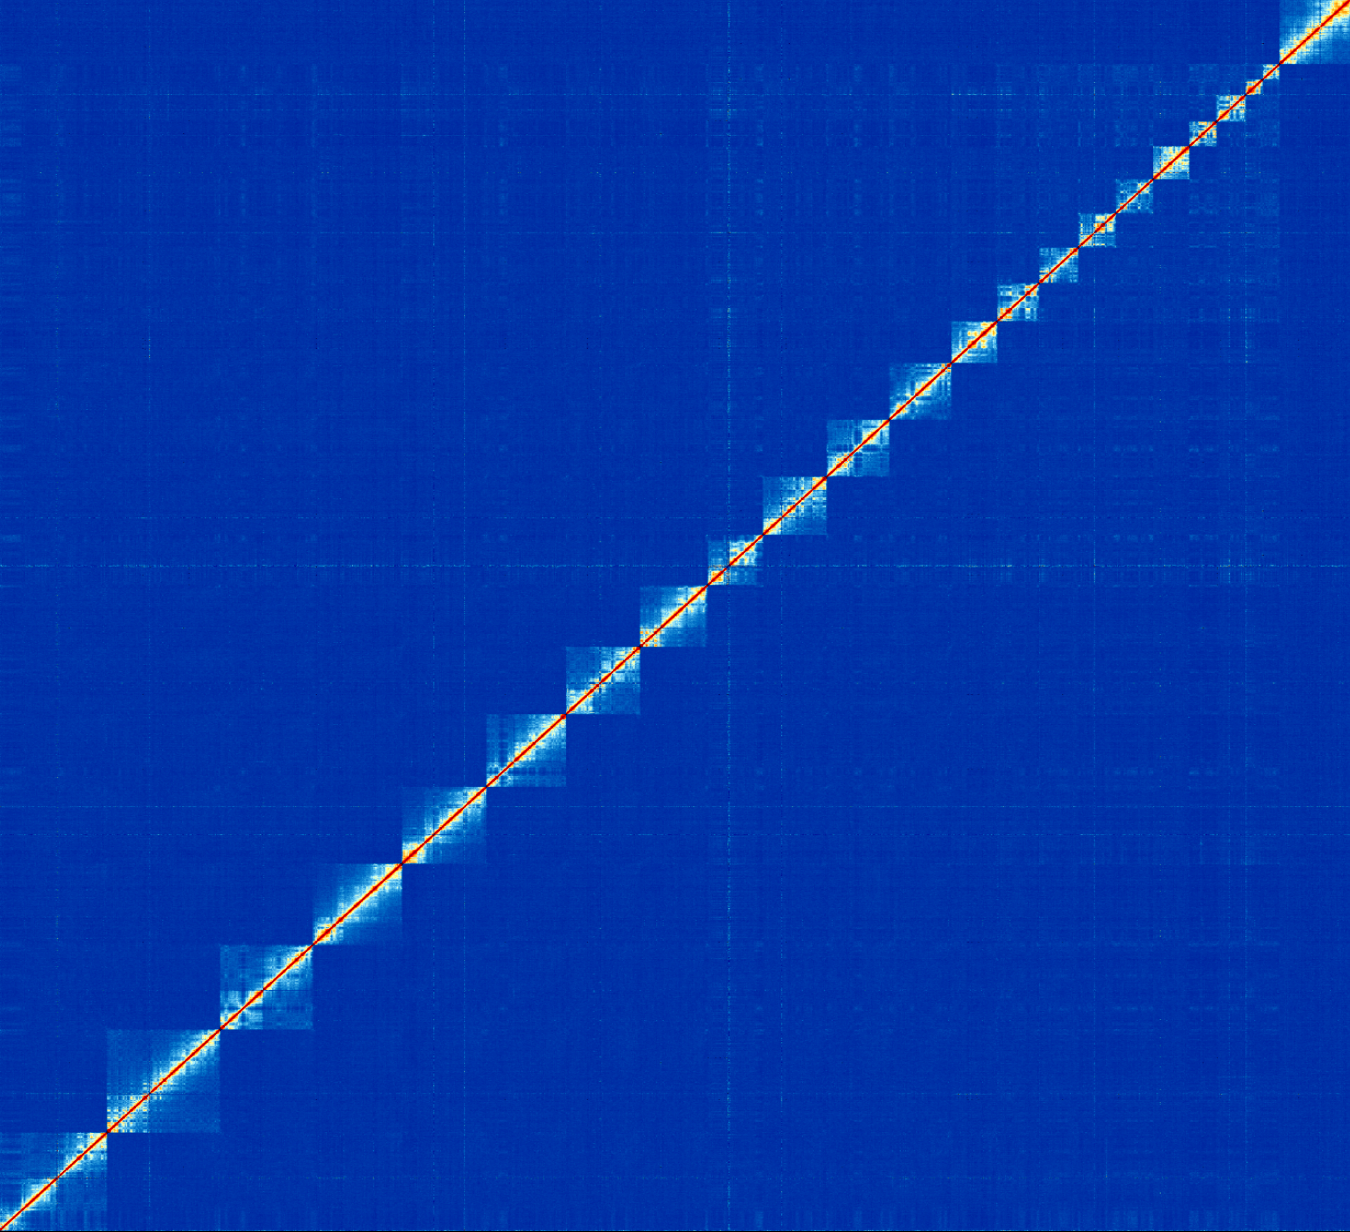
\includegraphics[width=.85\paperwidth]{figs/hicbg_3.png}}
\begin{frame}{}
\begin{tcolorbox}[colback=blue!40!black,colframe=blue!40!black]
\begin{center}
{\usebeamercolor[fg]{whitetext}
{\small Results 3: } \\
 Chromatin domain boundaries}
\end{center}
\end{tcolorbox}
\end{frame}
}

% ----- Begin boundaries

\begin{frame}{Boundaries}

TAD boundaries have been shown to be enriched for various epigenomic marks. \\

\vspace{2em}

\begin{itemize}
\item Which of these boundary enrichments are statistically significant relative to a null model?
\item Are the same features enriched at chromatin compartment boundaries?
\item Are these enrichments shared across cell types?
\end{itemize}

\end{frame}

\begin{frame}{Boundary enrichment analysis}

\centering

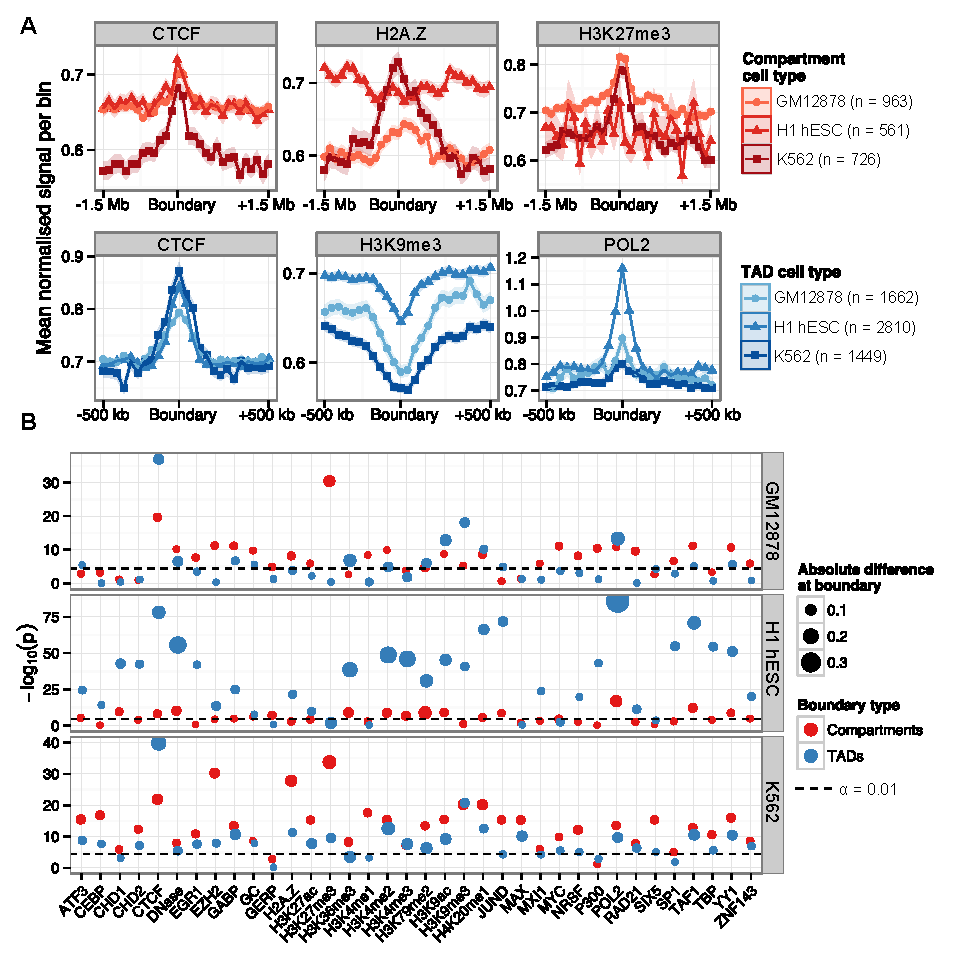
\includegraphics[width=.8\textwidth]{../figs/boundarysummary.pdf}

\end{frame}

\begin{frame}{Predicting TAD boundaries}{p96}

Given these enrichments exist, can we predict TAD boundaries in lieu of Hi-C data using epigenomic features? \\

\vspace{2em}

\centering
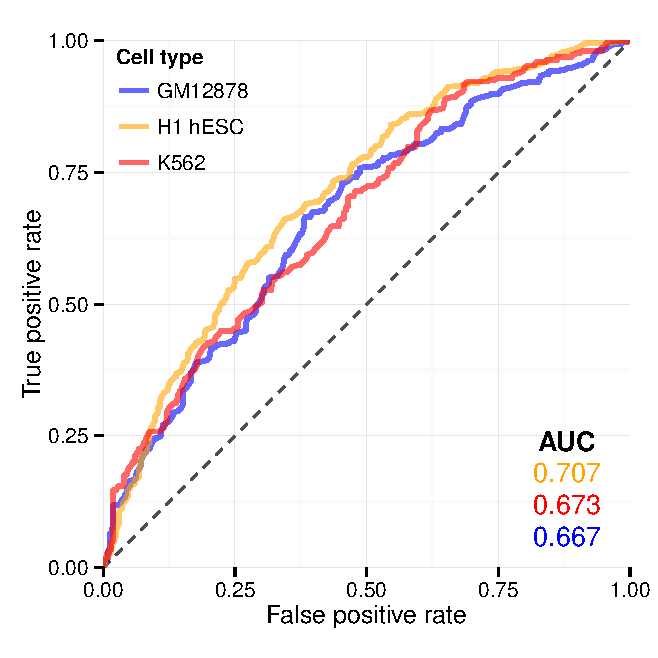
\includegraphics[width=.5\textwidth]{../figs/tadpred_auroc.pdf}


\end{frame}

\begin{frame}{Predicting TAD boundaries}

In this case, more consistent and clear results from variable importance:

\vspace{2em}

\centering
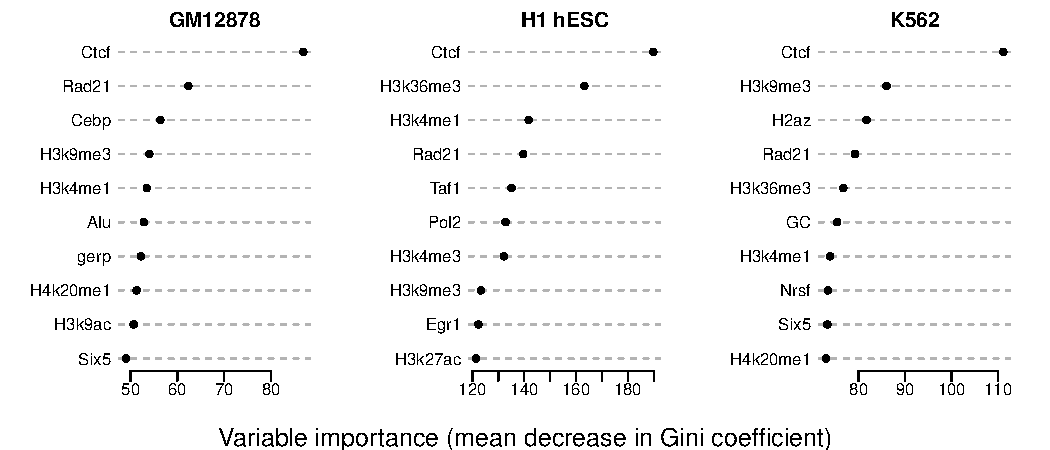
\includegraphics[width=\textwidth]{../figs/tadpred_varimp.pdf}

\end{frame}


\begin{frame}{MetaTADs}

Collaborator's finding: \\
\begin{quote}
Neighbour joining of interacting TADs appears to 
capture a novel layer of chromatin organisation: metaTADs. This attractive
concept that offers a framework for fractal 3D structure and links TADs with compartments.
 \end{quote}

\vspace{2em}

My contributions: \\
\begin{itemize}
\item Analysis of MetaTAD boundary enrichments as per TADs and compartments
\item Analysis of the co-incidence of MetaTAD boundaries and LAD boundaries
\end{itemize}

\vspace{2em}

\end{frame}

\begin{frame}{MetaTAD boundary enrichments}{p100}

\centering
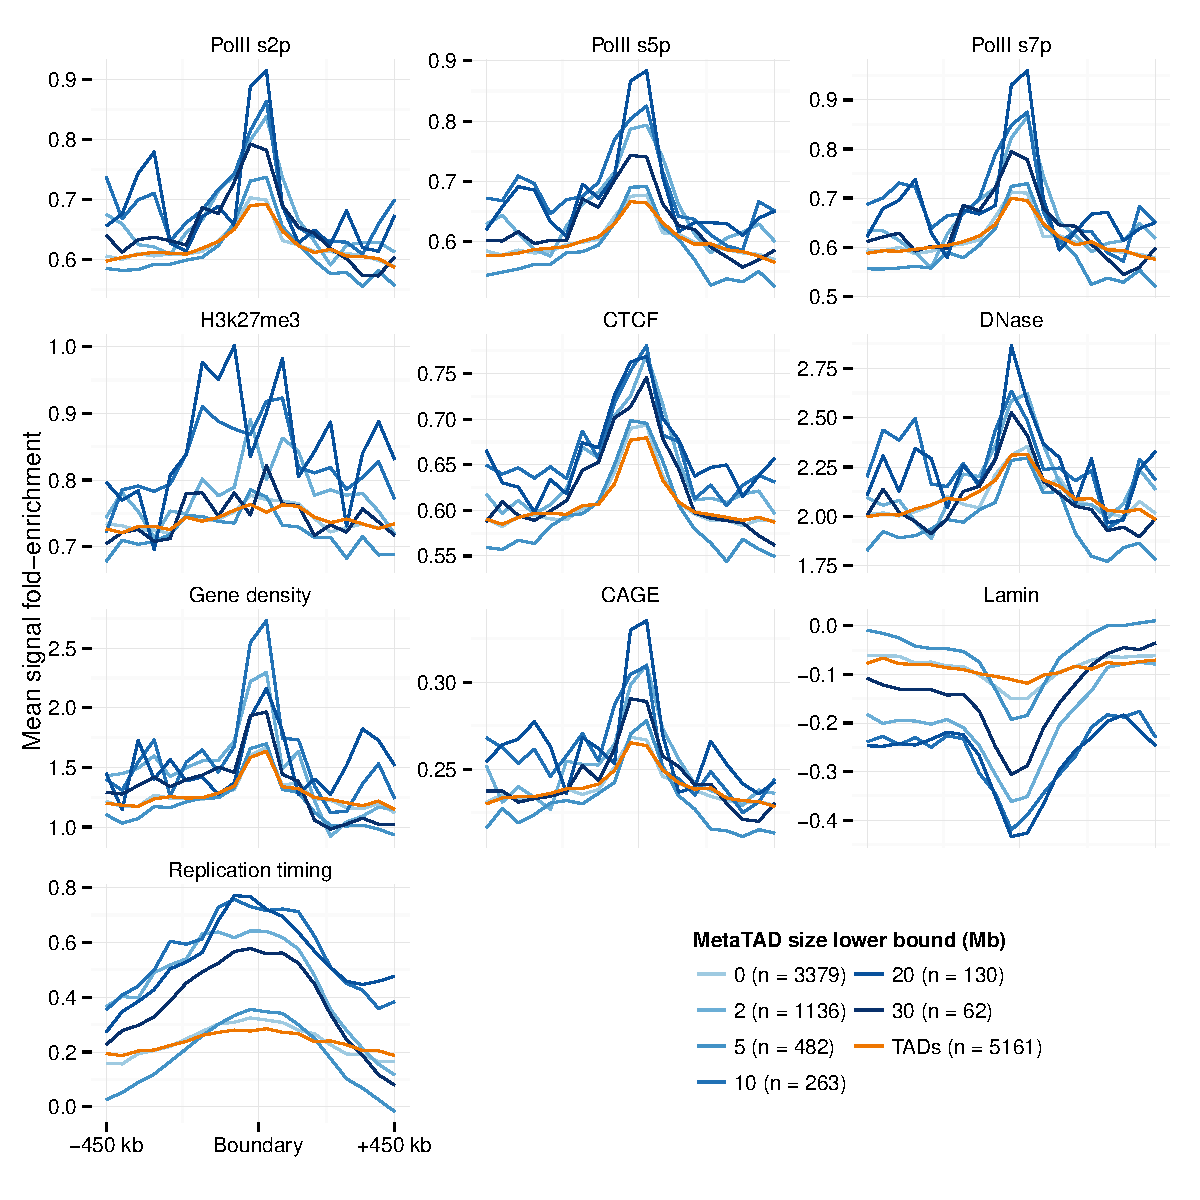
\includegraphics[width=.75\textwidth]{../figs/metatad_cutoffenrich.pdf}

\end{frame}

\begin{frame}{MetaTADs and LADs}{p100}

Are lamin associated domains being captured as metaTADs?

\centering
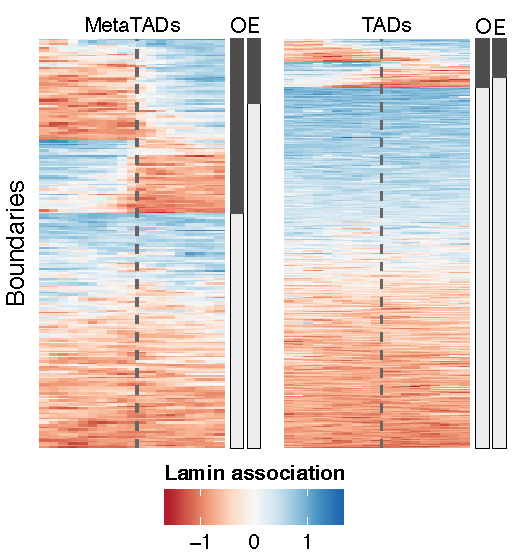
\includegraphics[width=.55\textwidth]{../figs/mt_laminsummary.pdf}

\end{frame}


\section{Local chromatin conformation}
{
\usebackgroundtemplate{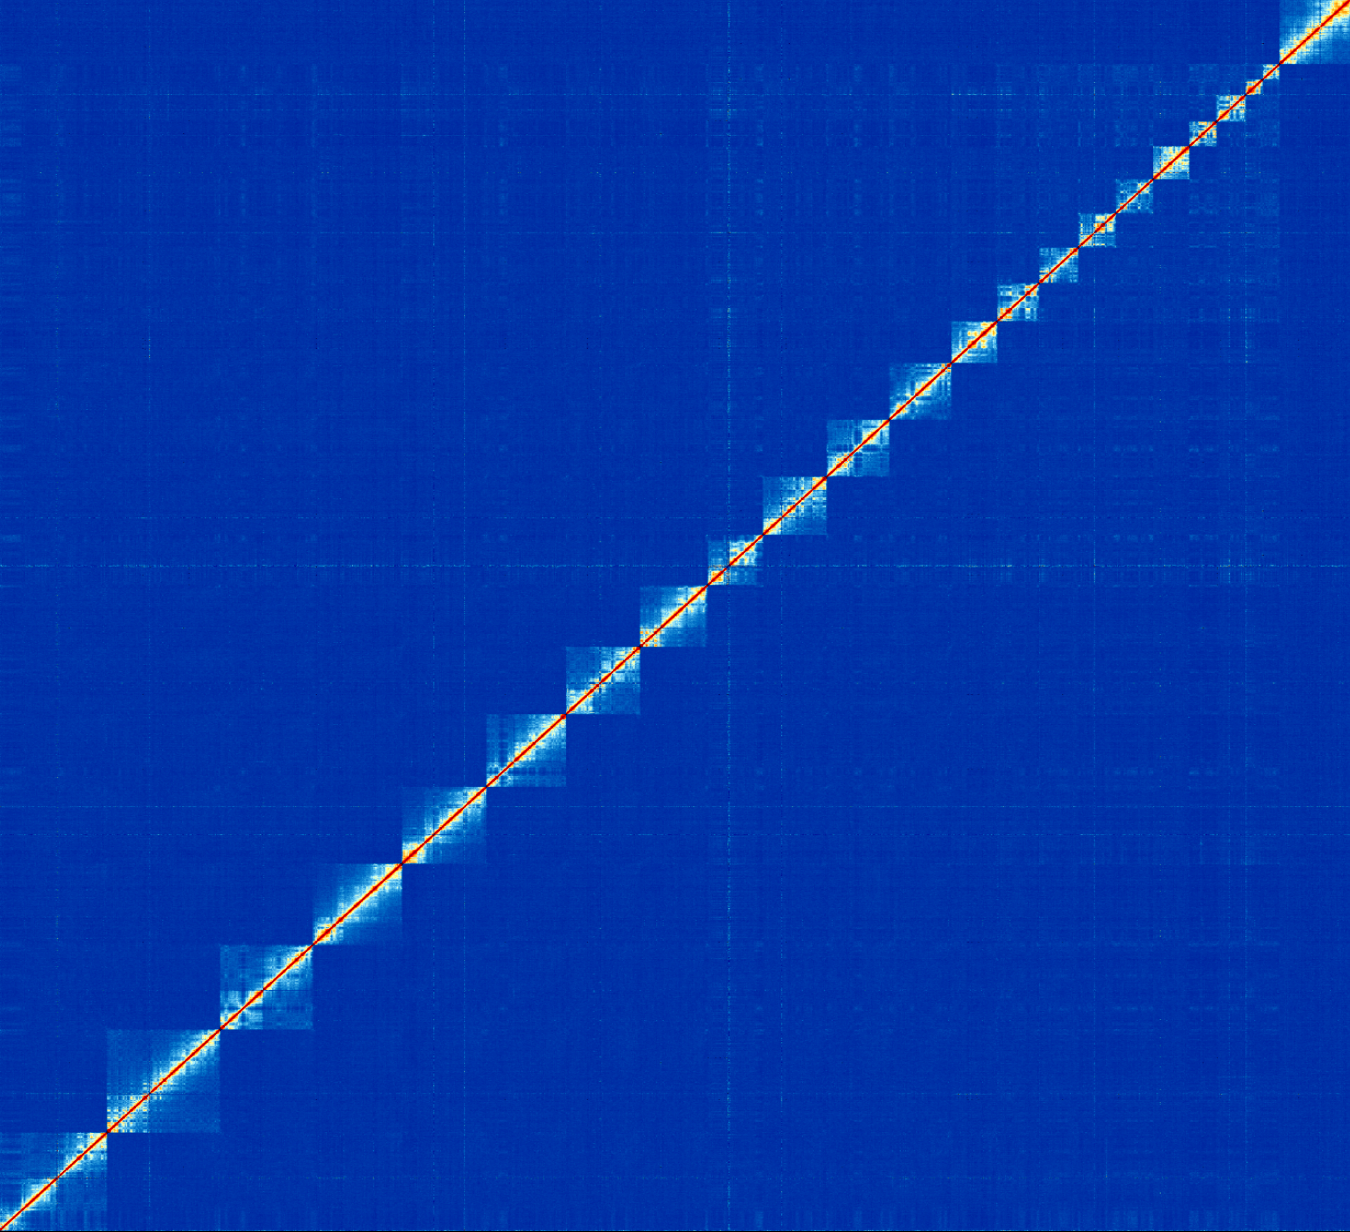
\includegraphics[width=.85\paperwidth]{figs/hicbg_3.png}}
\begin{frame}{}
\begin{tcolorbox}[colback=blue!40!black,colframe=blue!40!black]
\begin{center}
{\usebeamercolor[fg]{whitetext}
{\small Results 4: } \\
Local chromatin conformation }
\end{center}
\end{tcolorbox}
\end{frame}
}

% ----- Begin Local chromatin conformation

\begin{frame}{Local chromatin conformation}
Collaboration w/ Adam Douglas (Bob Hill's group) in analysing his
3C-seq (4C) data. Their experimental question: \\

\vspace{1em}

\centerline{
\includegraphics[width=.65\textwidth]{figs/tsa.png}
}

My contribution: analysis of 4C, 5C data and inference of 3D chromatin trajectory

\end{frame}

\begin{frame}{Shh locus}

ZRS-\emph{Shh} is a model system for long range \emph{cis}-regulation through an enhancer--promoter contact

\vspace{1em}

\centerline{
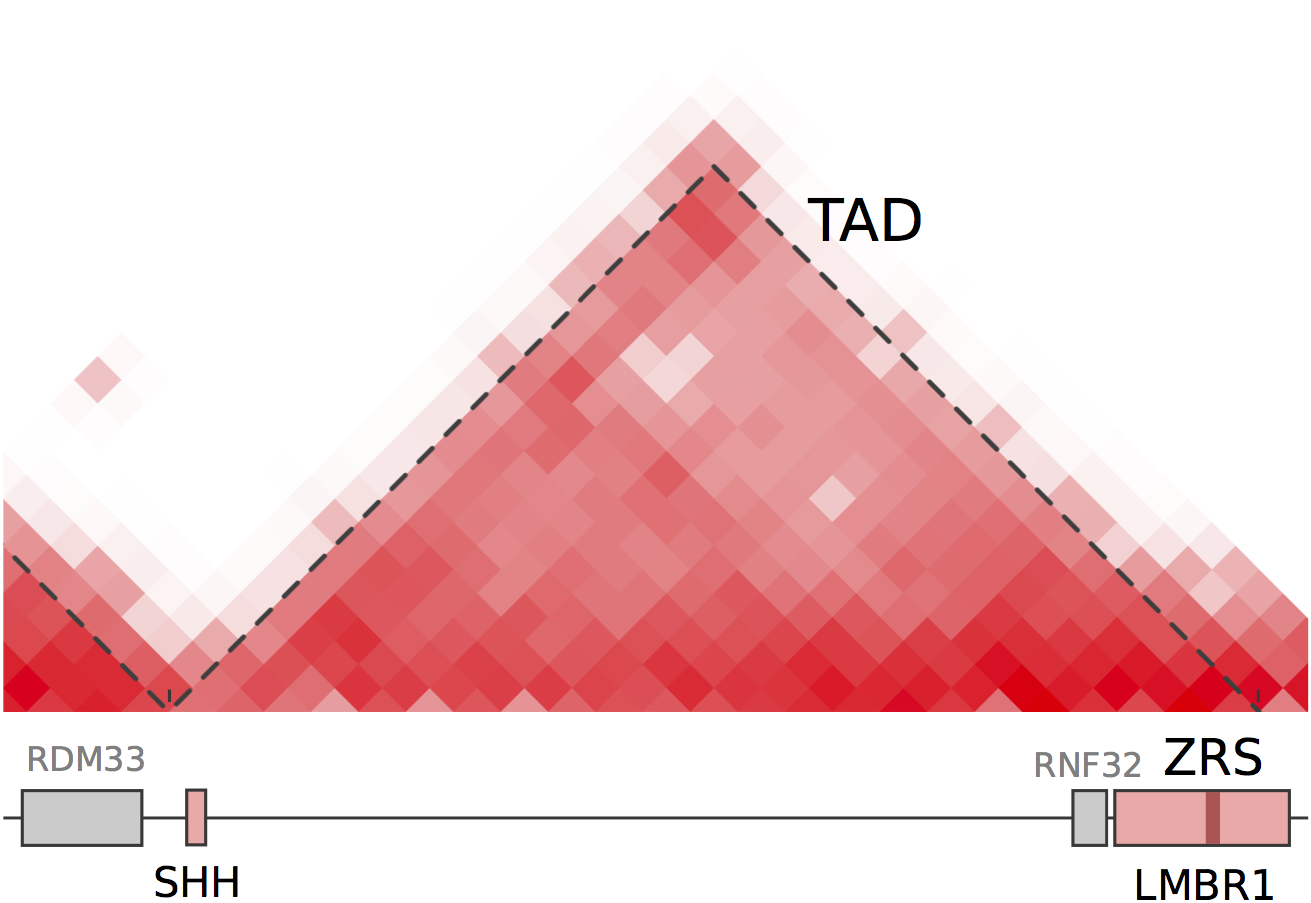
\includegraphics[width=.7\textwidth]{../figs/shhtad.png} 
} 

The Hill lab has developed an \emph{Shh}-inducible system through TSA treatment, though exact mechanism unclear

\end{frame}

\begin{frame}{4C results}{p112}

\centering
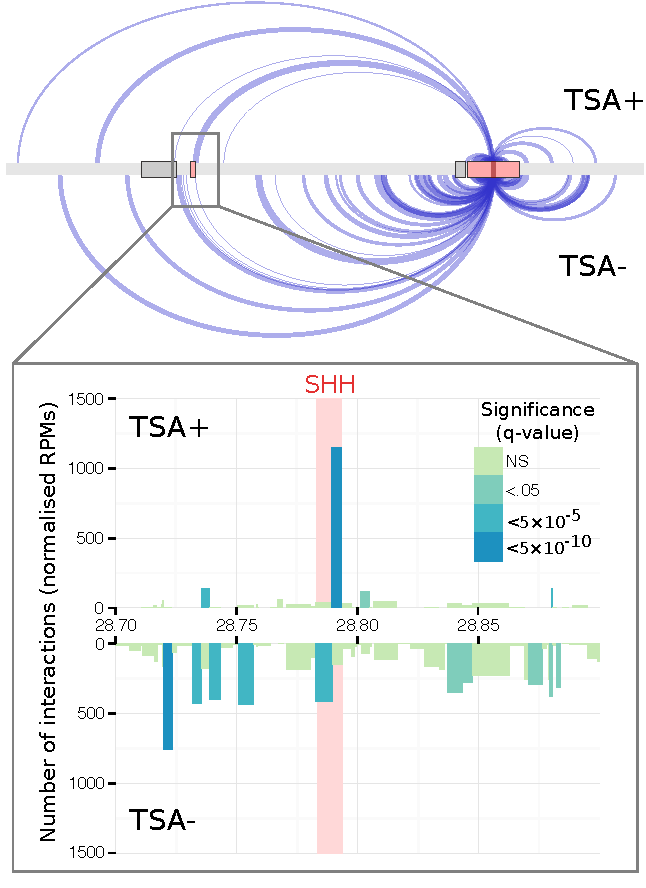
\includegraphics[width=.55\textwidth]{../figs/shharc_full.pdf} 

\end{frame}

\begin{frame}{5C results}{p118}

Used 5C data over the same region, passed to 3D reconstruction algorithm and measured distances \\

\centerline{
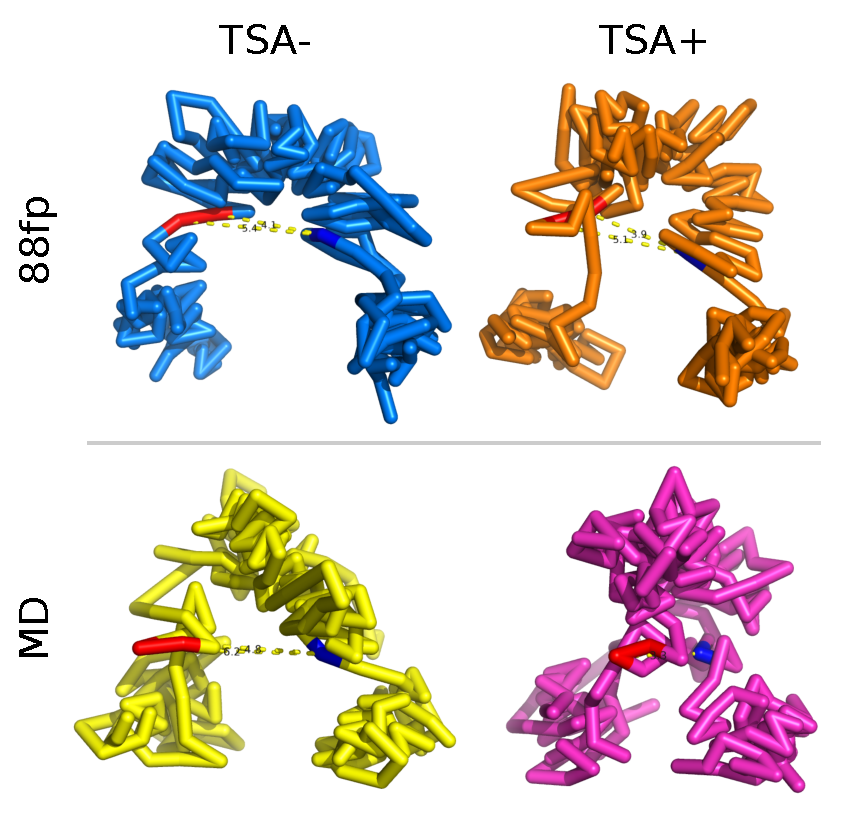
\includegraphics[width=.5\textwidth]{../figs/5c3d.pdf}
}
\vspace{1em}

Contrary to expectations, little change in inducible cell line and large shift in control mandibular cell line (non-\emph{shh} expressing)

\end{frame}

\begin{frame}{5C results}{p121}

Reconstructing TAD lends some credibility to the structures \\

\vspace{1em}

\centerline{
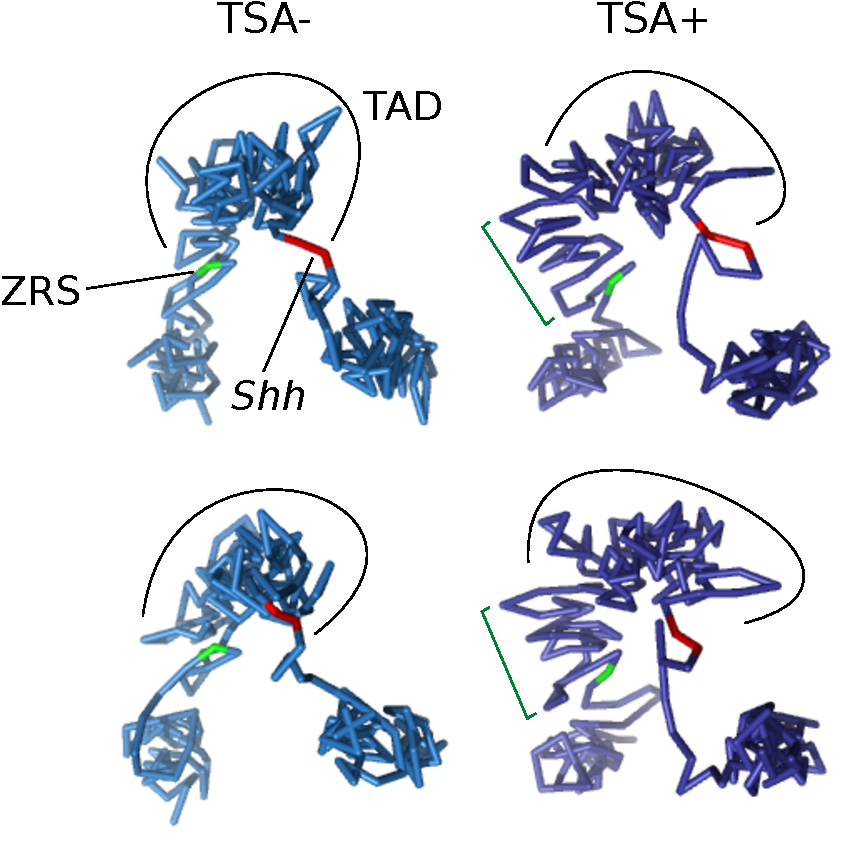
\includegraphics[width=.5\textwidth]{../figs/decompaction.pdf}
}
\vspace{1em}

HDAC causing some distension around ZRS in 14fp?

\end{frame}

\section{Discussion}

{
\usebackgroundtemplate{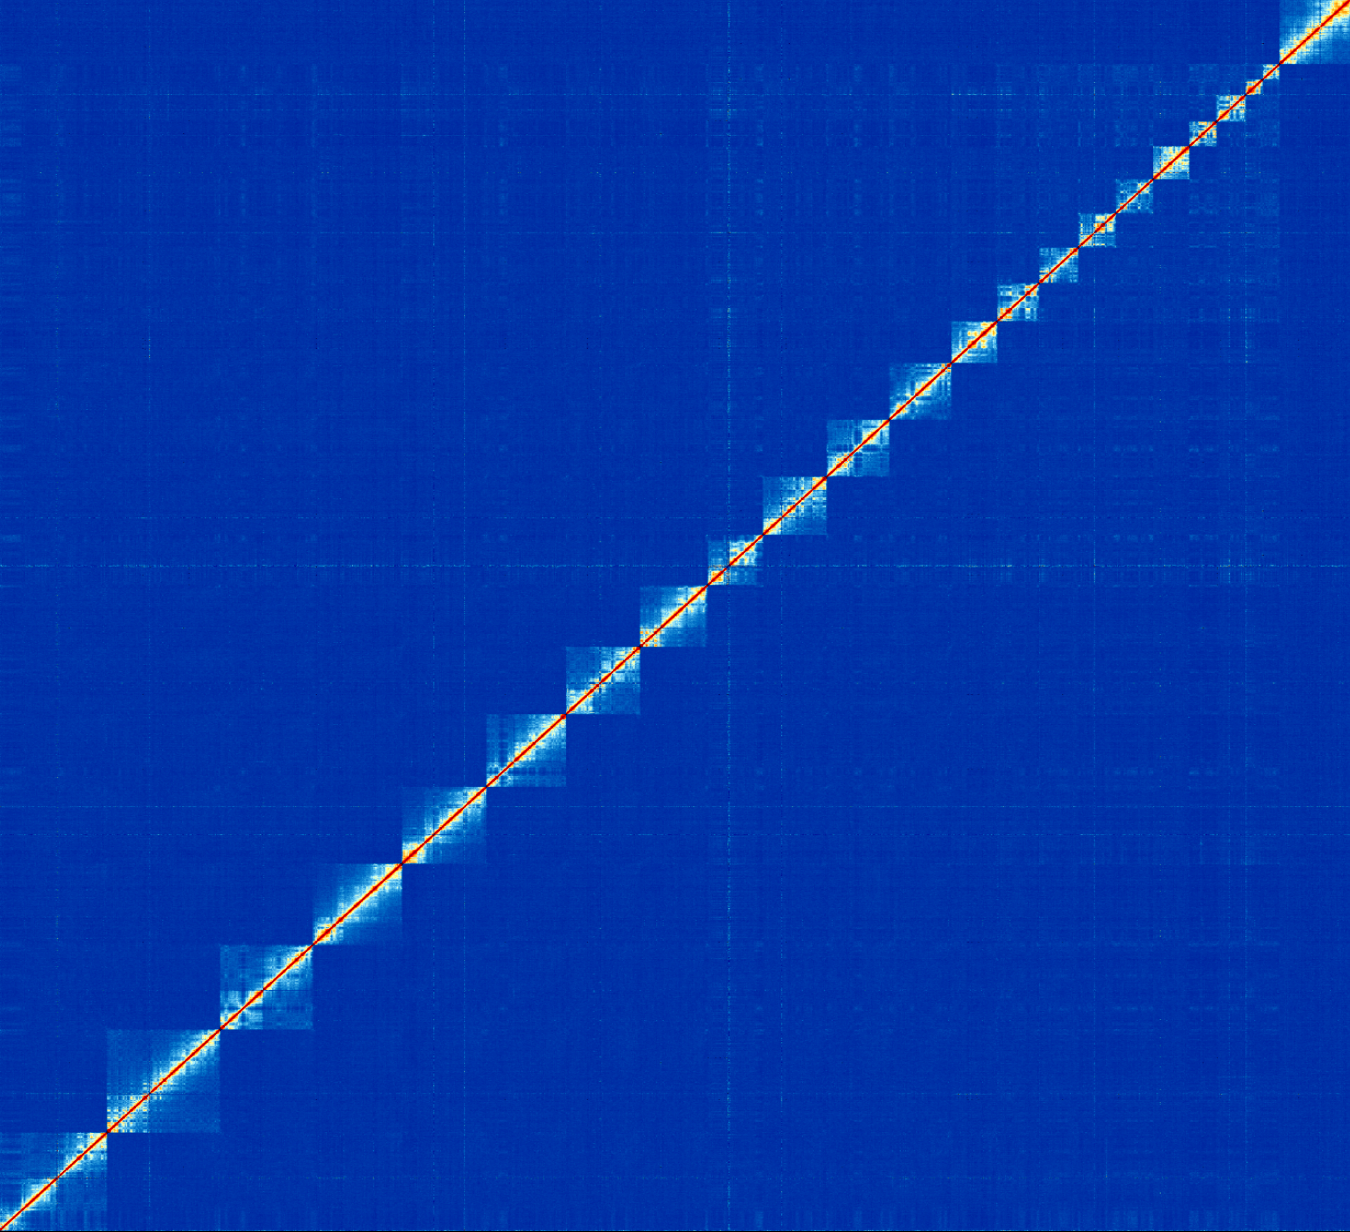
\includegraphics[width=.85\paperwidth]{figs/hicbg_3.png}}
\begin{frame}{}
\begin{tcolorbox}[colback=blue!40!black,colframe=blue!40!black]
\begin{center}
{\usebeamercolor[fg]{whitetext}
Discussion and Summary }
\end{center}
\end{tcolorbox}
\end{frame}
}

\begin{frame}{Discussion}{p123}

I suggest some extensions and discuss some open questions:
\begin{itemize}
\item Could a multi-tiered model predict TADs, MetaTADs and compartments from epigenomic data?
\item Are boundaries important or a side-effect of domains? (Likely something inbetween)
\end{itemize} 

\vspace{2em}

Ultimately our results agree with a model of genome organisation where large constitutive structures (compartments, LADs) anchor the genome but more local, cell-type specific interactions can then fine-tune transcriptional events at a local level

\end{frame}
%

\begin{frame}{Summary}

\small

Results presented in this thesis:
\begin{itemize}
\item Chromosome compartments can be accurately predicted from epigenomic features alone
\item This link between locus-level epigenomics and higher order structure is particularly evident at boundary regions
\item Further evidence for combinatorial importance of CTCF, YY1, RAD21 in genome organisation
\item MetaTADs appear a useful and biologically-relevant novel organisational strata
\item TSA inducible \emph{Shh} expression intimately linked with chromosome conformation, through details still unclear
\end{itemize}
\vspace{.5em}
More generally:
\begin{itemize}
\item Data recycling: most of this thesis done with publicly-available data from different sources
\item Machine learning offers useful tools to dissect complex biological systems
\end{itemize}
 
 
\end{frame}

\section{Acknowledgements}

{
\usebackgroundtemplate{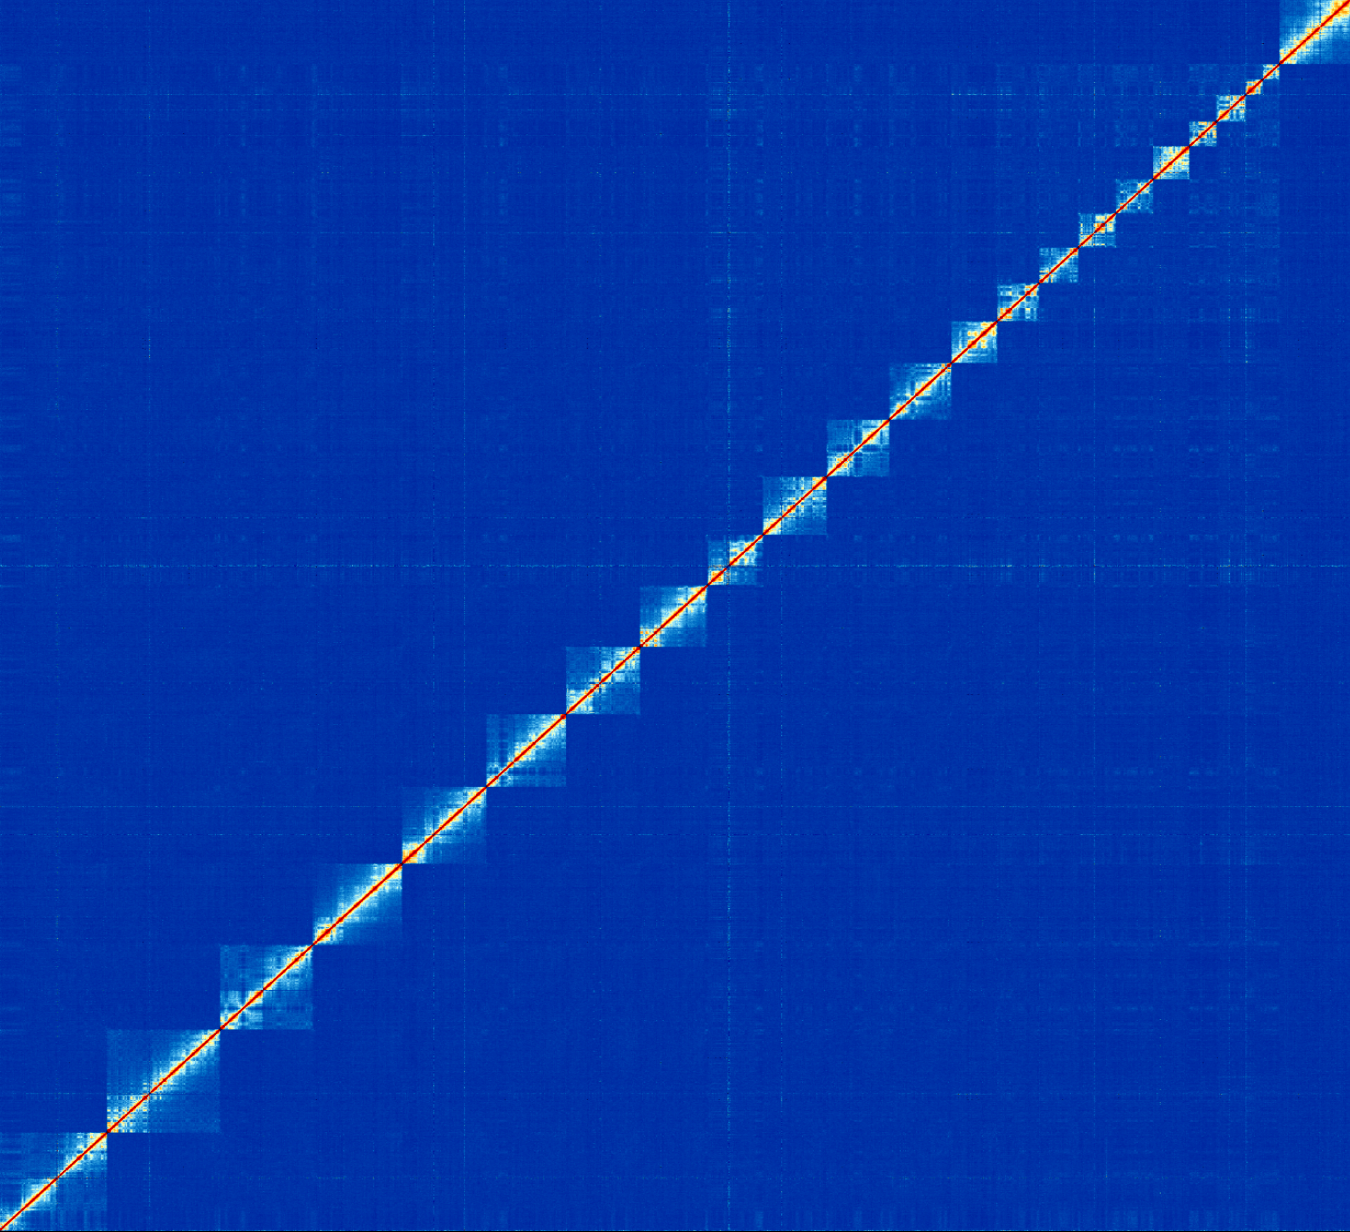
\includegraphics[width=.85\paperwidth]{figs/hicbg_3.png}}
\begin{frame}{}
\begin{tcolorbox}[colback=blue!40!black,colframe=blue!40!black]
\begin{center}
{\usebeamercolor[fg]{whitetext}
{\small Thanks to supervisors:} \\ 
Colin Semple and
Stuart Aitken \\
\vspace{1em}
{\small Collaborators:} \\
Hill lab (University of Edinburgh) \\ 
Pombo lab (Max Delbr\"uck center)

}

\end{center}
\end{tcolorbox}

\end{frame}
}


\end{document}